\documentclass[10pt, a4paper]{article}
\usepackage{preamble}

\newcommand{\mbf}[1]{\mathbf{#1}}
\newcommand{\ts}[1]{\textsuperscript{#1}}

\title{Linear Algebra I}
\author{Luke Phillips}
\date{October 2024}

\begin{document}

\maketitle

\newpage

\section{Vectors and vector spaces}

\subsection{Vector space $\R ^ n$}

\begin{definition}
    $n$-dimensional real space $\R ^ n$ a set of elements as such\[
    \R ^ n = \left\{\underline{x} = \begin{pmatrix}
        x_1 \\
        x_2 \\
        \vdots \\
        x_n
    \end{pmatrix}
    \quad:\ x_i \in \R
    \right\}\footnote{Vectors are $\underline{x}$ or $\mbf{x}$.}\]
\end{definition}

\begin{definition}
    The zero vector is defined as
    \[
    \mbf{0} = \begin{pmatrix}
        0 \\
        0 \\
        \vdots \\
        0
    \end{pmatrix}
    \in \R ^ n
    \]
\end{definition}

There are two operations on $\R ^ n$

\textbf{Vector addition}:

Vector addition is a function defined as such
\[
\R ^ n \times \R ^ n \mapsto \R ^ n
\]
This function takes two vectors $\mbf{v, w}$ and obtains
\[
(\mbf{v, w})\mapsto \mbf{v + w}
\]
For example
\[
\mbf{v + w} = \begin{pmatrix}
    v_1 \\
    v_2 \\
    \vdots \\
    v_n
\end{pmatrix} + \begin{pmatrix}
    w_1 \\
    w_2 \\
    \vdots \\
    w_n
\end{pmatrix}
=
\begin{pmatrix}
    v_1 + w_1 \\
    v_2 + w_2 \\
    \vdots \\
    v_n + w_n
\end{pmatrix}
=
\mbf{v + w}
\]

\textbf{Scalar multiplication}:

Scalar multiplication is defined as a function
\[
\R \times \R ^ n \mapsto \R ^ n.
\]
This is written as follows
\[
(\lambda, \mbf{v}) \mapsto \lambda\mbf{v}
\]
The operation is defined as such
\[
\lambda\mbf{v} = \lambda\begin{pmatrix}
    v_1 \\
    v_2 \\
    \vdots \\
    v_n
\end{pmatrix}
=
\begin{pmatrix}
    \lambda v_1 \\
    \lambda v_2 \\
    \vdots \\
    \lambda v_n
\end{pmatrix}
\]

\textbf{Intuition}

Vectors can be thought of a point in $n$-dimensional space
\begin{figure}[h!]
    \centering
    \begin{tikzpicture}
    \draw[->] (0,0) -- (0,2);
    \draw[->] (0,0) -- (2,0);
    \draw[->] (0,0) -- (1.5,1);
    \filldraw (1,1) circle (2pt);
    \end{tikzpicture}
    \caption{Graph 1}
    \label{fig:Gr1}
\end{figure}

As a direction to a point
\begin{figure}[h!]
    \centering
    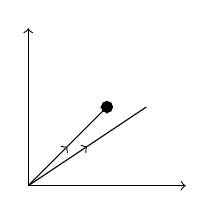
\begin{tikzpicture}
    \draw[->] (0,0) -- (0,2);
    \draw[->] (0,0) -- (2,0);
    \draw[->] (0,0) -- (0.75,0.5);
    \draw[-] (0.75,0.5) -- (1.5,1);
    \draw[->] (0,0) -- (0.5, 0.5);
    \draw[->] (0.5,0.5) -- (1, 1);
    \filldraw (1,1) circle (2pt);
    \end{tikzpicture}
    \caption{Graph 2}
    \label{fig:Gr2}
\end{figure}

As up to translation
\begin{figure}[h!]
    \centering
    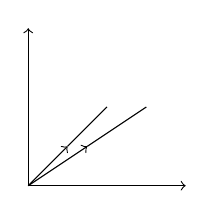
\begin{tikzpicture}
    \draw[->] (0,0) -- (0,2);
    \draw[->] (0,0) -- (2,0);
    \draw[->] (0,0) -- (0.75,0.5);
    \draw[-] (0.75,0.5) -- (1.5,1);
    \draw[->] (0,0) -- (0.5, 0.5);
    \draw[-] (0.5,0.5) -- (1, 1);
    \end{tikzpicture}
    \caption{Graph 3}
    \label{fig:Gr3}
\end{figure}

Vector addition
\begin{figure}[h!]
    \centering
    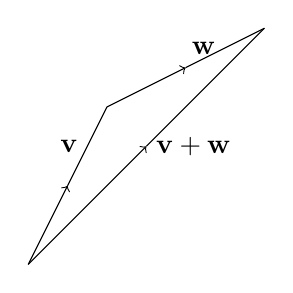
\begin{tikzpicture}
    \draw[->] (0,0) -- (0.5,1);
    \draw[-] (0.5,1) -- (1,2) node [midway, left] {$\mbf{v}$};
    \draw[->] (1,2) -- (2,2.5);
    \draw[-] (2,2.5) -- (3,3) node [midway, left] {$\mbf{w}$};
    \draw[->] (0,0) -- (1.5,1.5) node [right] {$\mbf{v + w}$};
    \draw[-] (1.5,1.5) -- (3,3);
    \end{tikzpicture}
    \caption{Graph 4}
    \label{fig:Gr4}
\end{figure}

Scalar multiplication
\begin{figure}[h!]
    \centering
    \begin{tikzpicture}
    \draw[->] (2,2) -- (3,3) node[left] {$\mbf{v}$};
    \draw[-] (3,3) -- (4,4);
    \draw[->] (2,0) -- (4,2) node[left] {$\mbf{\lambda v}$};
    \draw[->] (4,2) -- (6,4);
    \end{tikzpicture}
    \caption{Graph 5}
    \label{fig:Gr5}
\end{figure}
\textbf{Gr5}


These operations satisfy the \textbf{axioms} of a real vector space.
\begin{enumerate}[label = (\roman*)]
    \item There exists an additive identity $\mbf{0} \in \R ^ n$ such that
    \[
    \mbf{0 + v = v + 0 = v} \ \forall \mbf{v} \in \R ^ n.
    \]
    \item Commutativity
    \[
    \forall\mbf{w, v} \in \R ^ n\quad\mbf{w + v =  v + w}
    \]
    \item Existence of additive inverses
    \[
    \forall\mbf{v} \in \R ^ n\ \exists\mbf{-v} \in \R ^ n \text{ s.t. } \mbf{v + (-v) = (-v) + v = 0}
    \]
    \item Associativity
    $\forall\mbf{u, v, w} \in \R ^ n$
    \[
    (\mbf{u + v}) + \mbf{w} = \mbf{u} + (\mbf{v + w})
    \]
\end{enumerate}
(i), (iii), (iv) $\iff (\R ^ n, +)$ is a group

(i), (ii), (iii), (iv) $\iff (\R ^ n, +)$ is an abelian group \\


\textbf{Axioms} for scalar multiplication
\begin{enumerate}[label = (\roman*)]
    \item $0\mbf{v} = \mbf{0}\quad\forall\mbf{v}\in \R ^ n$.
    \item $1\mbf{v} = \mbf{v}\quad\forall\mbf{v}\in \R ^ n$.
    \item Associativity
    \[
    \lambda (\mu\mbf{v}) = (\lambda\mu)\mbf{v}\quad\forall\lambda,\mu \in \R\quad\forall\mbf{v}\in\R ^ n
    \]
    \item Distributivity, $\forall\lambda,\mu\in\R\quad\forall\mbf{v, w} \in \R ^ n$
    \begin{align*}
    (\lambda + \mu)\mbf{v} &= \lambda\mbf{v} + \mu\mbf{v} \\
    \lambda(\mbf{v + w}) &= \lambda\mbf{v} + \lambda\mbf{w}
    \end{align*}
\end{enumerate}

$\R ^ n$ clearly satisfies these axioms (if not obvious check) because they can be checked component-wise once we set 
\[
-\mbf{v} = \begin{pmatrix}
    -v_1 \\
    -v_2 \\
    \vdots \\
    -v_n
\end{pmatrix}
\]

\begin{definition}
    Standard basis vectors
    
    For $1 \leq i \leq n$ we define $\mbf{e}_i \in \R ^ n$
    \[
    \mbf{e}_i = \begin{pmatrix}
        0 \\
        0 \\
        \vdots \\
        0 \\
        1\footnote{$i$th position from the top.} \\
        0 \\
        \vdots \\
        0
    \end{pmatrix}
    \]    
\end{definition}

\begin{example}
    \[
    \mbf{e}_1 = \begin{pmatrix}
        1 \\
        0 \\
        \vdots \\
        0
    \end{pmatrix}
    \]
    \[
    \mbf{e}_2 = \begin{pmatrix}
        0 \\
        1 \\
        \vdots \\
        0
    \end{pmatrix}
    \]
\end{example}

We can express any vector $\mbf{x} \in \R ^ n$ uniquely as a linear combination of the standard basis vectors.

\begin{example}
    \begin{align*}
    \mbf{x} &= \begin{pmatrix}
        x_1 \\
        x_2 \\
        \vdots \\
        x_n
    \end{pmatrix}
    =
    x_1 \begin{pmatrix}
        1 \\
        0 \\
        \vdots \\
        0
    \end{pmatrix}
    +
    x_2 \begin{pmatrix}
        0 \\
        1 \\
        \vdots \\
        0
    \end{pmatrix}
    +
    \dots
    +
    x_n \begin{pmatrix}
        0 \\
        0 \\
        \vdots \\
        0 \\
        1
    \end{pmatrix} \\
    &= x_1 \mbf{e}_1 + x_2 \mbf{e}_2 + \dots + x_n \mbf{e}_n
    \end{align*}
\end{example}
The $x_i$'s are sometimes called the Cartesian coordinates of the vector $\mbf{x}$.

\subsection{The scalar (or dot) product in $\R ^ n$}

\begin{definition}
    The scalar product is defined as $\R ^ n \times \R ^ n \mapsto \R$, $(\mbf{u, v}) \mapsto \mbf{u \cdot v}$
    \begin{align*}
    \mbf{u \cdot v} &= \begin{pmatrix}
        u_1 \\
        u_2 \\
        \vdots \\
        u_n
    \end{pmatrix} \cdot
    \begin{pmatrix}
        v_1 \\
        v_2 \\
        \vdots \\
        v_n
    \end{pmatrix} \\
    &= u_1 v_1 + u_2 v_2 + \dots + u_n v_n  \\
    &= \sum_{i = 1}^{n}u_iv_i \in \R
    \end{align*}
\end{definition}

\begin{example}
    \[
    \begin{pmatrix}
        4 \\
        1 \\
        2
    \end{pmatrix}
    \cdot
    \begin{pmatrix}
        -3 \\
        -2 \\
        1
    \end{pmatrix}
    =
    -12 - 2 + 2 = -12.
    \]
\end{example}


\textbf{Axioms} of the scalar product
% To-Do add in the foralls here
\begin{enumerate}[label = (\roman*)]
    \item Symmetry
    \[
    \mbf{u \cdot v = v \cdot u}\qquad\forall\mbf{u, v} \in \R ^ n
    \]
    \item Linearity (1)
    \begin{align*}
    (\mbf{u + v)\cdot w}) &= \mbf{u \cdot w + v \cdot w}\qquad\forall \lambda \in \R\\
    \lambda\mbf{u})\cdot \mbf{w} &= \lambda (\mbf{u \cdot w})\qquad\forall\mbf{u, v, w} \in \R ^ n
    \end{align*}
    \item Linearity (2)
    \begin{align*}
        \mbf{u} \cdot (\mbf{v + w}) &= \mbf{u} \cdot \mbf{v} + \mbf{u} \cdot \mbf{w}\qquad \forall \lambda \in \R \\
        \mbf{u} \cdot \lambda\mbf{v} &= \lambda(\mbf{u \cdot v})\qquad \forall\mbf{u, v, w} \in \R ^ n
    \end{align*}
    \item Positivity
    \begin{align*}
        \mbf{v \cdot v} \geq 0\quad \forall \mbf{v} \in \R ^ n \\
        \text{and } \mbf{v \cdot v} = 0 \iff \mbf{v = 0}
    \end{align*}
\end{enumerate}

\begin{definition}
    Given a vector $\mbf{v} \in \R ^ n$ we define its magnitude (or length) to be
    \[
    |\mbf{v}| = \sqrt{\mbf{v \cdot v}}
    \]
\end{definition}
Note $\mbf{v \cdot v} \geq 0$ so positive square roots exist. Likewise note

$|\mbf{v}| \geq 0 \text{ and } |\mbf{v}| = 0 \iff \mbf{v = 0}$

\begin{example}
    \[
    \left|\begin{pmatrix}
        -3 \\
        4
    \end{pmatrix}\right|
    = \sqrt{(-3) ^ 2 + 4 ^ 2} = \sqrt{25} = 5
    \]
\end{example}

Thinking about a vector $\mbf{v} \in \R ^ 2$ where $\mbf{v \neq 0}$
\begin{figure}[h!]
    \centering
    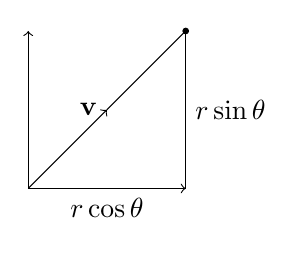
\begin{tikzpicture}
    \draw[->] (0,0) -- (0,2);
    \draw[->] (0,0) -- (2,0);
    \draw[->] (0,0) -- (1,1) node[left] {$\mbf{v}$};
    \draw[-] (1,1) -- (2,2);
    \draw[-] (2,0) -- (2,2) node[midway, right] {$r\sin\theta$};
    \draw[-] (0,0) -- (2,0) node[midway, below] {$r\cos\theta$};
    \filldraw (2,2) circle (1pt);
    \end{tikzpicture}
    \caption{Graph 9}
    \label{fig:Gr9}
\end{figure}

\[
\mbf{v}  = \begin{pmatrix}
    r\cos\theta \\
    r\sin\theta
\end{pmatrix}
\]
where
$r = |\mbf{v}|$ and $0 \leq \theta < 2\pi$, $\theta$ is the angle made by $\mbf{v}$ in an anticlockwise direction with the positive real axis.

We define $(r, \theta) \in (0, \infty) \times [0, 2\pi)$
to be the unique numbers such that
$\mbf{v}  = \begin{pmatrix}
    r\cos\theta \\
    r\sin\theta
\end{pmatrix}$
we call $(r, \theta)$ the polar coordinates of $\mbf{v}$

\begin{example}
    Suppose $\mbf{v} = \begin{pmatrix}
        2 \\
        3
    \end{pmatrix}$,
    what are its polar coordinates?

    $r = |\mbf{v}| = \sqrt{2 ^ 2 + 3 ^ 2} = \sqrt{13}$

    $\theta = \arcsin \left({\dfrac{3}{\sqrt{13}}}\right)$
\end{example}

\begin{example}
    Suppose $\mbf{v} = \begin{pmatrix}
        2 \\
        -2
    \end{pmatrix}$,
    what are its polar coordinates?

    $r = |\mbf{v}| = \sqrt{2 ^ 2 + (-2) ^ 2} = \sqrt{8} = 2\sqrt{2}$

    $\theta = \dfrac{7\pi}{4}$
\end{example}

\begin{proposition}
    Suppose $\mbf{v}, \mbf{w} \in \R ^ n$
    \[
    |\mbf{v}| = r,\quad|\mbf{w}| = s
    \]
    Suppose that $\mbf{v}, \mbf{w}$ make an angle of $\alpha$ with each other $0 \leq \alpha \leq \pi$
    
    Then $\mbf{v}\cdot\mbf{w} = rs\cos(\alpha)$.
    \begin{proof}
        Suppose polar coordinated of $\mbf{v}$ are $(r, \theta)$, and of $\mbf{w}$ are $(s, \varphi)$.

        Then $\mbf{v} = \begin{pmatrix}
            r\cos\theta \\
            r\sin\theta
        \end{pmatrix}$, $\mbf{w} = \begin{pmatrix}
            s\cos\varphi \\
            s\sin\varphi
        \end{pmatrix}$
        \begin{align*}
        \mbf{v\cdot w} &= \begin{pmatrix}
            r\cos\theta \\
            r\sin\theta
        \end{pmatrix} \cdot \begin{pmatrix}
            s\cos\varphi \\
            s\sin\varphi
        \end{pmatrix} \\
        &= rs\cos\theta\cos\varphi + rs\sin\theta\sin\varphi \\
        &= rs(\cos\theta\cos\varphi + \sin\theta\sin\varphi) \\
        &= rs(\cos(\theta - \varphi) \\
        &= rs\cos(\pm\alpha) = rs\cos\alpha.
        \end{align*}
    \end{proof}
\end{proposition}

\begin{corollary}
    If $\mbf{v} \neq \mbf{0}$ and $\mbf{w} \neq \mbf{0}$.
    $\mbf{v}$ and $\mbf{w}$ are orthogonal if and only if
    \[
    \mbf{v \cdot w} = 0.
    \]
    \begin{proof}
        \[
        \mbf{v \cdot w} = 0 \iff \cos(\alpha) = 0 \iff \alpha = \frac{\pi}{2}
        \]
    \end{proof}
\end{corollary}

\begin{example}
    $\mbf{v} = \begin{pmatrix}
        6 \\
        -2
    \end{pmatrix}\qquad
    \mbf{w} = \begin{pmatrix}
        -1 \\
        -3
    \end{pmatrix}$

    Then $\mbf{v\cdot w} = 6(-1) + (-2)(-3) = 0$

    So $\mbf{v, w}$ are orthogonal.
\end{example}


\begin{theorem}[Cauchy-Schwarz inequality]
    Suppose $\mbf{u, v} \in \R ^ n$, $\mbf{u, v} \neq 0$ then we have
    \[
    |\mbf{u}||\mbf{v}| \geq |\mbf{u \cdot v}|
    \]
    with equality if and only if $\mbf{u, v}$ are parallel (multiples of each other).
\end{theorem}

\begin{definition}
    Suppose $\mbf{u, v} \in \R ^ n$ with $\mbf{u, v \neq 0}$ then we define the angle between them to be the unique $0 \leq \theta \leq \pi$ such that $\mbf{u \cdot v} = |\mbf{u}||\mbf{v}|\cos\theta$.
\end{definition}

\begin{example}
    Find the angle between the vectors 
    \[
    \mbf{v} = \begin{pmatrix}
        1 \\ 2 \\ 1 \\ 3
    \end{pmatrix}, \quad \mbf{w} = \begin{pmatrix}
        1 \\ 3 \\ -1 \\ 3
    \end{pmatrix} \in \R ^ 4.
    \]
    Find $\theta$ s.t. $\mbf{v\cdot w} = |\mbf{v}||\mbf{w}|\cos\theta$

    $|\mbf{v}| = \sqrt{1 ^ 2 + 2 ^ 2 + 1 ^ 2 + 3 ^ 2} = \sqrt{1 + 4 + 1 + 9} = \sqrt{15}$
    
    $|\mbf{w}| = \sqrt{1 ^ 2 + 3 ^ 2 + (-1) ^ 2 + 3 ^ 2} = \sqrt{1 + 9 + 1 + 9} = \sqrt{20} = 2\sqrt{5}$

    $\mbf{v \cdot w} = 1 + 6 + -1 + 9 = 15$
    \[
    \cos\theta = \frac{\mbf{v \cdot w}}{|\mbf{v}||\mbf{w}|} = \frac{15}{\sqrt{15}\sqrt{20}} = \frac{\sqrt{15}}{\sqrt{20}} = \frac{\sqrt{3}}{\sqrt{4}} = \frac{\sqrt{3}}{2}
    \]
    $\theta = \dfrac{\pi}{6}$.
\end{example}

For $\mbf{v, w} \in \R ^ n$ $\mbf{v, w \neq 0}$ if $\mbf{v \cdot w} = 0$ (so they make an angle of $\frac{\pi}{2}$) we call $\mbf{v, w}$ orthogonal.

\begin{example}
    Find all unit\footnote{$|\mbf{w}| = 1$} vectors $\mbf{w} \in \R ^ 3$ that make an angle of $\frac{\pi}{4}$ with both.
    \[
    \mbf{u} = \begin{pmatrix} 1 \\ -1 \\ 0 \end{pmatrix},
    \quad\mbf{v} = \begin{pmatrix} 1 \\ 0 \\ 1 \end{pmatrix}.
    \]

    Suppose $\mbf{w} = \begin{pmatrix} w_1 \\ w_2 \\ w_3 \end{pmatrix}$ is a solution.

    First note $|\mbf{u}| = \sqrt{1 ^ 2 + (-1) ^ 2} = \sqrt{2}$,\quad$|\mbf{v}| = \sqrt{1 ^ 2 + 1 ^ 2} = \sqrt{2}$
    Now $\mbf{u \cdot w} = |\mbf{u}||\mbf{w}|\cos\left(\frac{\pi}{4}\right) = \sqrt{2} \cdot 1 \cdot \frac{1}{\sqrt{2}} = 1$

    and $\mbf{v \cdot w} = |\mbf{v}||\mbf{w}|\cos\left(\frac{\pi}{4}\right) = \sqrt{2} \cdot 1 \cdot \frac{1}{\sqrt{2}} = 1$.

    So $w_1 - w_2 = 1$ and $w_1 + w_3 = 1$. So $w_2 = w_1 - 1$ and $w_3 = 1 - w_1$.
    Also $\mbf{w \cdot w} = 1$ so $w_1 ^ 2 + w_2 ^ 2 + w_3 ^ 2 = 1$.
    Hence $w_1 ^ 2 + (w_1 - 1) ^ 2 + (1 - w_1) ^ 2 = 1$
    solve for $w_1$ (two solutions)
\end{example}

\subsection{The vector product}
The vector product (or cross product)
\[
\R ^ 3 \times \R ^ 3 \rightarrow \R ^ 3
\]
\[
(\mbf{u, v}) \mapsto \mbf{u \times v}
\]

\begin{definition}
    \[
    \mbf{x \times y} = \begin{pmatrix}
        x_1 \\ x_2 \\ x_3
    \end{pmatrix}
    \times
    \begin{pmatrix}
        y_1 \\ y_2 \\ y_3
    \end{pmatrix}
    =
    \begin{pmatrix}
        x_2 y_3 - x_3 y_2 \\
        x_3 y_1 - x_1 y_3 \\
        x_1 y_2 - x_2 y_1
    \end{pmatrix}
    \]
\end{definition}

\begin{example}
    \[
    \begin{pmatrix}
        7 \\ -4 \\ 2   
    \end{pmatrix}
    \times
    \begin{pmatrix}
        2 \\ 3 \\ -1
    \end{pmatrix}
    =
    \begin{pmatrix}
        (-4)(-1) - 2 \cdot 3 \\
        2 \cdot 2 - 7 \cdot (-1) \\
        7 \cdot 3 - (-4)(2)
    \end{pmatrix}
    =
    \begin{pmatrix}
        -2 \\ 11 \\ 29
    \end{pmatrix}
    \]
\end{example}

Properties of the cross product
\begin{enumerate}[label = (\roman*)]
    \item Anti-symmetry: $\mbf{u \times v} = -(\mbf{v \times u})$\quad$\forall\mbf{u, v} \in \R ^ 3$
    \item Linearity 1:
    $(\mbf{u + v} \times \mbf{w} = \mbf{u \times w} + \mbf{v \times w}$\quad$\forall\lambda \in \R$
    
    $(\lambda\mbf{u}) \times \mbf{v} = \lambda(\mbf{u \times v})$\quad$\forall\mbf{u, v, w} \in \R ^ 3$
    
    \item Linearity 2:
    $\mbf{u} \times (\mbf{v + w}) = \mbf{u \times v + u \times w}$\quad$\forall\lambda \in \R$
    
    $\mbf{u} \times (\lambda\mbf{v}) = \lambda\mbf{u \times w}$\quad$\forall\mbf{u, v, w} \in \R ^ 3$

    \item Orthogonality to the input
    \[
    \mbf{u \cdot (u \times v)} = 0 = \mbf{v \cdot (u \times v)}\quad\forall\mbf{u, v} \in \R ^ 3
    \]
\end{enumerate}
In other words $\mbf{u \times v}$ is orthogonal to $\mbf{u}$ and $\mbf{v}$.

\begin{lemma}
    Suppose that $\mbf{x, y} \in \R ^ 3$ are vectors of length $|\mbf{x}| = r > 0$, $|\mbf{y}| = s > 0$. Then
    \[
    |\mbf{x \times y}| = rs\sin\theta
    \]
    where $0 \leq \theta \leq \pi$ is the angle between $\mbf{x}$ and $\mbf{y}$.
    
    \begin{proof}
        \begin{align*}
            |\mbf{x\times y}| ^ 2 &= (\mbf{x} \times \mbf{y}) \cdot (\mbf{x} \times \mbf{y}) \\
            &= (x_2y_3 - x_3y_2) ^ 2 + (x_3y_1 - x_1y_3) ^ 2 + (x_1y_2 - x_2y_1) ^ 2 \\
            &= (x_1 ^ 2 + x_2 ^ 2 + x_3 ^ 2)(y_1 ^ 2 + y_2 ^ 2 + y_3 ^ 2) - (x_1y_1 + x_2y_2 + x_3y_3) ^ 2 \\
            &= r ^ 2 s ^ 2 - (\mbf{x \cdot y}) ^ 2 \\
            &= r ^ 2 s ^ 2 - r ^ 2 s ^ 2 \cos ^ 2\theta \\ 
            &= r ^ 2 s ^ 2 (1 - \cos ^ 2\theta) \\ 
            &= r ^ 2 s ^ 2 \sin ^ 2 \theta 
        \end{align*}
    \end{proof}
\end{lemma}

\begin{example}
    \[
    \left|\begin{pmatrix}
        7 \\ -4 \\ 2   
    \end{pmatrix}\right| = \sqrt{49 + 16 + 4} = \sqrt{69}
    \]
    \[
    \left|\begin{pmatrix}
        2 \\ 3 \\ -1
    \end{pmatrix}\right| = \sqrt{4 + 9 + 1} = \sqrt{14}
    \]
    \[
    \left|\begin{pmatrix}
        7 \\ -4 \\ 2   
    \end{pmatrix}
    \times
    \begin{pmatrix}
        2 \\ 3 \\ -1
    \end{pmatrix}\right| = \left|\begin{pmatrix}
        -2 \\ 11 \\ 29
    \end{pmatrix}\right| = \sqrt{4 + 121 + 861} = \sqrt{966}.
    \]
    If $\theta$ is the angle between $\begin{pmatrix}
        7 \\ -4 \\ 2   
    \end{pmatrix}$ and $\begin{pmatrix}
        2 \\ 3 \\ -1
    \end{pmatrix}$ we have $\sqrt{966} = \sqrt{69}\sqrt{14}\sin\theta$ so $\sin\theta = 1$ and $\theta = \frac{\pi}{2}$.
\end{example}

\subsection{Planes in $\R ^ 3$}

\textbf{The parametric form}

Let $\Pi \subseteq \R ^ 3$ be a plane. $\mbf{a} \in \Pi$, point on the plane $\Pi$. $\mbf{d}_1, \mbf{d}_2 \in \R ^ 3$ parallel to $\Pi$ but not parallel to each other (i.e. "collinear"). $\mbf{d}_1 \neq 0$, $\mbf{d}_2 \neq 0$.

To get to any point $\mbf{p} \in \Pi$, first travel to the point $\mbf{a} \in \Pi$ then along $\mbf{d}_1$ and $\mbf{d}_2$ some amount. So
\[
\Pi = \{\mbf{a} + \lambda_1\mbf{d}_1 + \lambda_2\mbf{d}_2\,|\,\lambda_1, \lambda_2 \in \R\}.
\]
$\lambda_1, \lambda_2$ are called "free variables"\footnote{Or "free parameters".}. \\

\textbf{Using the normal vector}

Let $\Pi \subseteq \R ^ 3$ be a plane. $\mbf{a} \in \Pi$, $\mbf{n}$ is a normal vector to $\Pi$, ($n \neq 0$), 
\begin{align*}
    \mbf{x} \in \Pi &\iff (\mbf{x - a}) \text{ is orthogonal to } \mbf{n} \\
    &\iff (\mbf{x - a}) \cdot \mbf{n} = 0 \\
    &\iff \mbf{x \cdot a} - \mbf{a \cdot n} = 0 \\ 
    &\iff \mbf{x \cdot a} = \mbf{a \cdot n} \\ 
    &\iff \mbf{x \cdot a} = \ell.
\end{align*}

\begin{align*}
    \Pi &= \{\mbf{x} \in \R ^ 3\,|\,\mbf{x\cdot a} = \mbf{a \cdot n}\} \\
    &= \{\mbf{x} \in \R ^ 3\,|\, \mbf{x \cdot n} = \ell\}.
\end{align*}

\textbf{Cartesian form}

((B) in coordinates)

If we write $\mbf{n} = \begin{pmatrix}
    a \\ b \\ c
\end{pmatrix},\ \mbf{x} = \begin{pmatrix}
    x \\ y \\ z
\end{pmatrix}$ then $\mbf{n \cdot x} = \ell$ can be written:
\[
ax + by + cz = \ell
\]
So
\[
\Pi = \left\{\begin{pmatrix}
    x \\ y \\ z
\end{pmatrix} \in \R ^ 3\,|\, ax + by + cz = \ell\right\}.
\]

\begin{example}
    Find the Cartesian description of the plane $\Pi$ that passes through $\begin{pmatrix}
        1 \\ -1 \\ 3
    \end{pmatrix}$ and is normal to the direction $\begin{pmatrix}
        5 \\ 2 \\ 1
    \end{pmatrix}$.

    $\mbf{n} = \begin{pmatrix}
        5 \\ 2 \\ 1
    \end{pmatrix},\, \mbf{a} = \begin{pmatrix}
        1 \\ -1 \\ 3
    \end{pmatrix} \in \Pi$.
    \begin{align*}
    \Pi &= \left\{ \begin{pmatrix}
        x \\ y \\ z
    \end{pmatrix} \in \R ^ 3\,|\, \mbf{x \cdot n = a \cdot n}\right\} \\
    &=\left\{\begin{pmatrix}
        x \\ y \\ z
    \end{pmatrix} \in \R ^ 3\,|\, 5x + 2y + z = 6\right\}
    \end{align*}
\end{example}

\begin{example}
    Find a normal vector to and a point on the plane
    \[
    6x - 5y + 3z = 30
    \]
    $\mbf{n} = \begin{pmatrix}
        6 \\ -5 \\ 3
    \end{pmatrix}$, $\mbf{a}$ can be any point on the plane e.g. $\begin{pmatrix}
        5 \\ 0 \\ 0
    \end{pmatrix},\,\begin{pmatrix}
        0 \\ -6 \\ 0
    \end{pmatrix} \text{ or } \begin{pmatrix}
        0 \\ 0 \\ 10
    \end{pmatrix}$
\end{example}

Parametric description from normal/Cartesian.

Suppose 
\begin{align*}
    \Pi &= \{\mbf{x} \in \R ^ 3 \,|\, \mbf{n\cdot x} = \ell\}
    &= \left\{\begin{pmatrix} x \\ y \\ z
    \end{pmatrix} \in \R ^ 3 \,|\, ax + by + cz = \ell\right\}
\end{align*}
where $\mbf{n} = \begin{pmatrix} a \\ b \\ c \end{pmatrix}$

If $c \neq 0$ then \[
ax + by + cz = \ell \iff z = \frac{\ell}{c} - \left(\frac{a}{c}\right)x - \left(\frac{b}{c}\right)y.
\]
So
\[
\Pi = \left\{ \begin{pmatrix}
    0 \\ 0 \\ \frac{\ell}{c}
\end{pmatrix} + x\begin{pmatrix}
    1 \\ 0 \\ -\frac{a}{c} 
\end{pmatrix} + y\begin{pmatrix}
    0 \\ 1 \\ -\frac{b}{c}
\end{pmatrix}\,:\, x, y \in \R \right\}
\]
(where $x, y$ are "free parameters")

Likewise similarly if $a \neq 0$ or $b \neq 0$ (cannot have $a = b = c = 0$)

\begin{example}
    Find parametric and Cartesian description of the plane $\Pi \subseteq \R ^ 3$ that passes through
    \[
    \mbf{a} = \begin{pmatrix}
        1 \\ 0 \\ 1
    \end{pmatrix}
    \quad
    \mbf{b} = \begin{pmatrix}
        2 \\ -1 \\ 3
    \end{pmatrix},
    \quad
    \mbf{c} = \begin{pmatrix}
        5 \\ 1 \\ 1
    \end{pmatrix}.
    \]

    Set $\mbf{d}_1 = \mbf{b - a} = \begin{pmatrix}
        1 \\ -1 \\ 2
    \end{pmatrix}$, $\mbf{d}_2 = \mbf{c - a} = \begin{pmatrix}
        4 \\ 1 \\ 0
    \end{pmatrix}$

    So $\Pi = \{\mbf{a} + \lambda_1 \mbf{d}_1 + \lambda_2 \mbf{d}_2\,|\, \lambda_1, \lambda_2 \in \R\}$

    $\mbf{n} = \mbf{d}_1 \times \mbf{d}_2$ then $\mbf{n}$ is normal to $\mbf{d}_1$ and $\mbf{d}_2$ and so is normal to $\Pi$.
    \[
    \mbf{n} = \begin{pmatrix}
        1 \\ -1 \\ 2
    \end{pmatrix}
    \times \begin{pmatrix}
        4 \\ 1 \\ 0
    \end{pmatrix}
    =
    \begin{pmatrix}
        -2 \\ 8 \\ 5
    \end{pmatrix}
    \]
    $\ell = \mbf{n \cdot a} = -2 + 5 = 3$.

    So we have
    \[
    \Pi = \left\{\begin{pmatrix}
        x \\ y \\ z
    \end{pmatrix} \in \R ^ 3\,|\, -2x + 8y + 5z = 3\right\}
    \]
\end{example}

\subsection{Lines}

\textbf{Parametric}

$L \subseteq \R ^ 3$. Take $\mbf{a} \in L$, $\mbf{d} \neq 0$ parallel to $L$. Then
\[
L = \{\mbf{a} +\lambda\mbf{d}\,|\, \lambda \in \R\}
\]

\textbf{Cartesian}

Set $\mbf{a} = \begin{pmatrix}
    a_1 \\ a_2 \\ a_3
\end{pmatrix},\quad\mbf{d} = \begin{pmatrix}
    d_1 \\ d_2 \\ d_3
\end{pmatrix}$


\[
\begin{pmatrix}
    x \\ y \\ z
\end{pmatrix} \in L \iff
\]
\begin{align*}
    a_1 + \lambda d_1 &= x \\
    a_2 + \lambda d_2 &= y \\
    a_3 + \lambda d_3 &= z
\end{align*}
for some $\lambda \in \R$

Suppose $d_1 \neq 0,\, d_2 \neq 0,\,d_3 \neq 0$ then
\[
\lambda = \frac{x - a_1}{d_1},\,\lambda = \frac{y - a_2}{d_2},\,\lambda = \frac{z - a_3}{d_3}.
\]

So
\[
\begin{pmatrix}
    x \\ y \\ z
\end{pmatrix} \in L \iff
\frac{x - a_1}{d_1} = \frac{y - a_2}{d_2} = \frac{z - a_3}{d_3}.
\]

So 
\[
L = \left\{\begin{pmatrix}
    x \\ y \\ z
\end{pmatrix} \in \R ^ 3 | \frac{x - a_1}{d_1} = \frac{y - a_2}{d_2} = \frac{z - a_3}{d_3}\right\}.
\]

If $d_1, d_2 \neq 0,\,d_3 = 0$ then $\lambda = \frac{x - a_1}{d_1} = \frac{y - a_2}{d_2},\, z = a_3$.

If $d_1 \neq 0,\,d_2 = d_3 = 0$ then $y = a_2,\, z = a_3$.


\textbf{Intersection of two planes}

Suppose $\Pi_i = \{\mbf{x} \in \R ^ 3 \,|\, n_i \cdot \mbf{x} = \ell_i\}$ for $i = 1, 2$. Then, what is
\[
Pi_1 \cap \Pi_2 = \{\mbf{x}\in \R ^ 3 \,|\, \mbf{n}_1 \cdot \mbf{x} = \ell_1,\,\mbf{n}_2 \cdot \mbf{x} = \ell_2\}.
\]

If $\mbf{n}_1$ and $\mbf{n}_2$ are parallel (collinear) then either $\Pi_1 = \Pi_2$ or if $\Pi_1 \neq \Pi_2$ then $\Pi_1 \cap \Pi_2 = \emptyset$.

If $\mbf{n}_1$ and $\mbf{n}_2$ are not parallel then $\Pi_1 \cap \Pi_2 = L$ for some line $L$

So 
\[L = \{\mbf{x}\in \R ^ 3 \,|\, \mbf{n}_1 \cdot \mbf{x} = \ell_1,\,\mbf{n}_2 \cdot \mbf{x} = \ell_2\} = \left\{\begin{pmatrix}
    x \\ y \\ z
\end{pmatrix} \in \R ^ 3\, \middle|\,
    ax + by + cz = \ell_1,
    dx + ey + fz = \ell_2
\right\}
\]

Given a description of $L$ as in the intersection of two planes, how do we get the parametric description of $L$?
We need $\mbf{a} \in L,\,\mbf{d \neq 0}$ where $\mbf{d}$ is parallel to $L$.

$\mbf{d}$ is parallel to $\Pi_1$ and $\Pi_2$ so $\mbf{d} \cdot \mbf{n}_1 = 0$, and $\mbf{d} \cdot \mbf{n}_2 = 0$ so set $\mbf{d} = \mbf{n}_1 \times \mbf{n}_2 = \begin{pmatrix}
    a \\ b \\ c
\end{pmatrix} \times \begin{pmatrix}
    d \\ e \\ f
\end{pmatrix} = \begin{pmatrix}
    bf - ce \\
    cd - af \\
    ae - bd
\end{pmatrix}$.

To find $\mbf{a} \in L$

If $ae - bd \neq 0$ then

$\mbf{d}$ has some "$z$-component",

so $L$ intersects the $(x, y)$-plane at a unique point $\mbf{a} = \begin{pmatrix}
    g \\ h \\ 0
\end{pmatrix}$

$g, h$ satisfy
\begin{align*}
    ag + bh + 0 &= \ell_1 \\
    dg + eh + 0 &= \ell_2
\end{align*}
Solve for $g, h$.

\textbf{Points in} $\R ^ 3$

Suppose we have three planes
$\Pi_1,\,\Pi_2,\,\Pi_3 \subseteq \R ^ 3$.
\[
\Pi_i = \{x \in \R ^ 3 \, | \, \mbf{n}_i \cdot \mbf{x} = \ell_i\}\quad i = 1, 2, 3
\]

What are the possibilities for $\Pi_1 \cap \Pi_2 \cap \Pi_3$?
\begin{enumerate}[label = (\roman*)]
    \item A plane $(\Pi_1 = \Pi_2 = \Pi_3)$.
    \item A line $L$.
    \item A point.
    \item The empty set.
\end{enumerate}

When do we have the generic case (iii)?

Firstly we certainly want $\Pi_2 \cap \Pi_3$ to be a line $L$. So $\mbf{n}_1$ and $\mbf{n}_2$ cannot be parallel. And $L$ has direction vector
\[
\mbf{d} = \mbf{n}_2 \times \mbf{n}_3.
\]
Then we want to have that $L \cap \Pi_1 = \{\text{pt}\}.$ A set consisting of a single point. And this happens exactly when $L$ is not parallel to $\Pi_1$, i.e. $\mbf{d}$ is not orthogonal to $\mbf{n}_1$ i.e. $\mbf{n}_1 \cdot \mbf{d} \neq 0 \iff \mbf{n}_1 \cdot (\mbf{n}_2 \times \mbf{n}_3) \neq 0$.

\subsection{Scalar triple product}

\begin{definition}[Scalar triple product]
    The scalar triple product is a function
    \[
    \R ^ 3 \times \R ^ 3 \times \R ^ 3 \rightarrow \R
    \]
    \[
    (\mbf{a}, \mbf{b}, \mbf{c}) \mapsto [\mbf{a}, \mbf{b}, \mbf{c}].
    \]
    Where
    \[
    [\mbf{a}, \mbf{b}, \mbf{c}] := \mbf{a} \cdot (\mbf{b} \times \mbf{c}).
    \]
\end{definition}

\[
\mbf{a} = \begin{pmatrix}
    a_1 \\ a_2 \\ a_3
\end{pmatrix}\quad\mbf{b} = \begin{pmatrix}
    b_1 \\ b_2 \\ b_3
\end{pmatrix}\quad\mbf{c} = \begin{pmatrix}
    c_1 \\ c_2 \\ c_3
\end{pmatrix}.
\]
The system of equations
\begin{align*}
    a_1 x + a_2 y + a_3 z &= \ell_1 \\
    b_1 x + b_2 y + b_3 z &= \ell_2 \\
    c_1 x + c_2 y + c_3 z &= \ell_3
\end{align*}
$\ell_1, \ell_2, \ell_3 \in \R$.
Has a unique solution if and only if
\[
[\mbf{a}, \mbf{b}, \mbf{c}] \neq 0
\]

\begin{proposition}[Invariance under cyclic permutation]
    If $\mbf{a, b, c} \in \R ^ 3$ then
    \[
    [\mbf{a}, \mbf{b}, \mbf{c}] = [\mbf{b}, \mbf{c}, \mbf{a}] = [\mbf{c}, \mbf{a}, \mbf{b}] = -[\mbf{b}, \mbf{a}, \mbf{c}] = -[\mbf{a}, \mbf{c}, \mbf{b}] = -[\mbf{c}, \mbf{b}, \mbf{a}].
    \]
    \begin{proof}
        \begin{align*}
        [\mbf{a}, \mbf{b}, \mbf{c}] &= \mbf{a} \cdot \left(\begin{pmatrix}
            b_1 \\ b_2 \\ b_3
        \end{pmatrix} \times
        \begin{pmatrix}
            c_1 \\ c_2 \\ c_3
        \end{pmatrix}\right) \\
        &= \begin{pmatrix}
            a_1 \\ a_2 \\ a_3
        \end{pmatrix}
        \cdot
        \begin{pmatrix}
            b_2 c_3 - b_3 c_2 \\ b_3 c_1 - b_1 c_3 \\ b_1 c_2 - b_2 c_1
        \end{pmatrix} \\
        &= a_1 b_2 c_3 + a_2 b_3 c_1 + a_3 b_1 c_2 - a_1 b_3 c_2 - a_2 b_1 c_3 - a_3 b_2 c_1.
        \end{align*}
        This is invariant under cyclic permutations (and gets a minus sign under swaps).
    \end{proof}
\end{proposition}

Aside:
\[
[\mbf{a}, \mbf{b}, \mbf{c}] = \det\underbrace{\left(\mbf{a}\, \mbf{b}\, \mbf{c}\right)}_{3 \times 3 \text{ matrix}.}
\]

\newpage

\section{Matrices}

\begin{definition}[$m \times n$ matrix]
    An $m \times n$ matrix is a rectangular array of real numbers with $m$ rows and $n$ columns. We call the set of all $m \times n$ matrices
    \[
    M_{m \times n}(\R).
    \]
\end{definition}

We call the entry in position $(i,\,j)$ the $(i,\,j)$th element.

\begin{example}
    \[
    \begin{pmatrix}
        1 & 5 & 10 \\
        2 & 3 & 4
    \end{pmatrix} \in M_{2 \times 3}(\R).
    \]
    $(2, 3)$ entry is $4$

    $(1, 1)$ entry is $1$
\end{example}

If $A \in M_{m \times n}(\R)$ we write $A_{ij}$ or $a_{ij}$ for the $(i,\,j)^{\text{th}}$ entry or element. For shorthand we write $A = (a_{ij})_{m \times n}$.

Sometimes we write
\[
A = (f(i, j))_{m \times n} \text{ or } A = (f(i, j))
\]

\begin{example}
    $(i - j)_{3 \times 2} = \begin{pmatrix}
        1 - 1 = 0 & 1 - 2 = -1 \\
        1 & 0 \\
        2 & 1
    \end{pmatrix}
    =
    \begin{pmatrix}
        0 & -1 \\
        1 & 0 \\
        2 & 1
    \end{pmatrix}$
\end{example}

We call $M_{n \times 1}(\R) = \R ^ n$ a set of column vectors. We call $M_{1 \times n}(\R)$ a set of row vectors.

\underline{Transpose}

The transpose operation is a function 
\[
M_{m \times n}(\R) \rightarrow M_{n \times m}(\R)
\]
$A \mapsto A ^ t$
\[
(A ^ t)_{ij} = A_{ji}\text{ for } 1 \leq i \leq n, 1 \leq j \leq m.
\]

\begin{example}
    \[
    A = \begin{pmatrix}
        1 & 2 & 4 \\
        7 & 10 & 11
    \end{pmatrix}
    \]
    \[
    A ^ t = \begin{pmatrix}
        1 & 7 \\ 
        2 & 10 \\
        4 & 11
    \end{pmatrix}
    \]
\end{example}

\begin{definition}
    The zero matrix, written as $0_{m \times n} = 0 \in M_{m \times n}(\R)$ is defined by
    \[
    (0_{m \times n})_{ij} = 0\ \forall i,j
    \]
\end{definition}

\begin{definition}
    The Kronecker delta is a function
    \[
    \delta : \Z \times \Z \rightarrow \{0, 1\}.
    \]
    \[
    \delta_{ij} = \delta(i, j) = \begin{cases}
        1 &\text{if } i = j \\
        0 &\text{if } i \neq j
    \end{cases}
    \]
\end{definition}

\begin{definition}
    The $n \times n$ identity matrix $I_n \in M_{n \times n}(\R)[=M_n(\R) \text{ "square matrices"}]$ is defined by
    \[
    I_n = (\delta_{ij})_{n \times n} = \begin{pmatrix}
        1 & 0 & 0 & \dotsc & 0 & 0 \\
        0 & 1 & 0 & \dotsc & 0 & 0 \\
        0 & 0 & 1 & \dotsc & 0 & 0 \\
        \vdots & \vdots & \vdots & \ddots & \vdots & \vdots \\
        0 & 0 & 0 & \dotsc & 1 & 0 \\
        0 & 0 & 0 & \dotsc & 0 & 1
    \end{pmatrix}.
    \]
\end{definition}

\subsection{Matrix Operations}
Two basic operations:
\begin{enumerate}[label = (\roman*)]
    \item Matrix addition
    
    This is a function
    \[
    M_{m \times n}(\R) \times M_{m \times n}(\R) \rightarrow M_{m \times n}(\R)
    \]
    \[
    (X, Y) \mapsto X + Y.
    \]
    Defined by $(X + Y)_{ij} = X_{ij} + Y_{ij}$.

    \item Scalar multiplication

    This is a function
    \[
    \R \times M_{m \times n}(\R) \rightarrow M_{m \times n}(\R)
    \]
    \[
    (\lambda, X) \mapsto \lambda X.
    \]
    Defined by $(\lambda X)_{ij} = \lambda X_{ij}$
\end{enumerate}

\begin{example}
    \[
    \begin{pmatrix}
        1 & 2 & 3 \\ 5 & 6 & 7
    \end{pmatrix}
    +
    \begin{pmatrix}
        1 & 0 & 1 \\ 0 & 1 & 0
    \end{pmatrix}
    = \begin{pmatrix}
        2 & 2 & 4 \\ 5 & 7 & 7
    \end{pmatrix}
    \]
    \[
    3 \begin{pmatrix}
        1 & 2 & 3 \\ 5 & 6 & 7
    \end{pmatrix} = \begin{pmatrix}
        3 & 6 & 9 \\ 15 & 18 & 21
    \end{pmatrix}
    \]
\end{example}

\underline{Properties of these operations}

Addition
\begin{enumerate}[label = (\roman*)]
    \item Additive identity. There exists a $0_{m \times n} \in M_{m \times n}(\R)$ such that $0_{m \times n} + X = X = X + 0_{m \times n}\ \forall x \in M_{m \times n}(\R)$.
    \item Commutativity.
    \[
    X + Y = Y + X\quad \forall X, Y \in M_{m \times n}(\R).
    \]
    \item Additive inverses
    \[
    \forall X \in M_{m \times n}(\R)\ \exists -X \in M_{m \times n}(\R)
    \]
    such that $X + (-X) = 0_{m \times n} = (-X) + X$.

    \item Associativity.
    \[
    (X + Y) + Z = X + (Y + Z)\quad\forall X, Y, Z \in M_{m \times n}(\R).
    \]
\end{enumerate}

Scalar multiplication
\begin{enumerate}[label = (\roman*)]
    \item $0X = 0_{m\times n}\quad\forall X \in M_{m \times n}(\R)$.
    \item $1X = X\quad\forall X \in M_{m \times n}(\R)$.
    \item Associativity
    \[
    \lambda(\mu X) = (\lambda \mu) X\quad \forall \lambda, \mu \in \R, \forall X \in M_{m \times n}(\R) 
    \]
    \item Distributivity
    \[
    (\lambda + \mu)X = \lambda X + \mu X
    \]
    \[
    \lambda(X + Y) = \lambda X + \lambda Y
    \]
    $\forall \lambda \mu \in \R, \forall X, Y \in M_{m \times n}(\R)$.
\end{enumerate}

\subsection{Matrix Multiplication}

\begin{definition}
    Matrix multiplication is a function
    \[
    M_{m \times n}(\R) \times M_{n \times p}(\R) \rightarrow M_{m \times p}(\R)
    \]
    \[
    (X, Y) \mapsto XY
    \]
    Suppose $X = (x_{ij}),\, Y = (y_{ij})$. Then
    \[
    (XY)_{ij} = \sum_{k = 1}^{n}x_{ik}y_{kj} = x_{i1}y_{1j} + x_{i2}y_{j2} + \dotsc + x_{in}y_{nj}. 
    \]
    "Multiplying the rows of $X$ and the columns of $Y$".
\end{definition}

Properties of matrix multiplication

$X, X' \in M_{m \times n}(\R),\quad Y, Y' \in M_{n \times p}(\R),\, Z \in M_{p \times r}(\R)$, $\forall \lambda, \lambda' \in \R$ we have:
\begin{enumerate}[label = (\roman*)]
    \item $0_{p \times m}X = 0_{p \times n} = Z0_{r \times n}$.
    \item $I_{m}X = X = XI_{n}$.
    \item $\lambda(XY) = (\lambda X)Y = X(\lambda Y)$.
    \item $(XY)Z = X(YZ)$
    
    \item 
    \begin{align*}
        (X + X')Y &= XY + X'Y \\
        X(Y + Y') &= XY + XY' \\
        \lambda(X + X') &= \lambda X + \lambda X' \\
        (\lambda + \lambda')X &= \lambda X + \lambda' X.
    \end{align*}
\end{enumerate}
\begin{proof}
    \begin{enumerate}[label = (\roman*)]
        \item \phantom{}
        \item \phantom{}
        \item \phantom{}
        \item What is the $(i,\,j)$th entry of $(XY)Z$?

        The $(i,\,k)$th entry of $XY$ is $(XY)_{ik} = \sum_{r = 1}^{n}x_{ir}y_{rk}$
        Then
        \[
        ((XY)Z)_{ij} = \sum_{k = 1}^{p}\overbrace{\left(\sum_{r = 1}^{n}x_{ir}y_{rk}\right)}^{(XY)_{ik}}z_{kj}
        \]
        The $(r,\,j)$th entry of $YZ$ is
        \[
        \sum_{k = 1}^{p}y_{rk}z_{kj},
        \]
        so the $(i,\,j)$th entry of $X(YZ)$ is $\displaystyle\sum_{r = 1}^{n}x_{ir}\left(\sum_{k = 1}^{p}y_{rk}z_{kj}\right) = \sum_{r = 1}^{n}\sum_{k = 1}^{p}x_{ir}y_{rk}z_{kj} = \sum_{k = 1}^{p}\left(\sum_{r = 1}^{n}x_{ir}y_{rk}\right)z_{kj}$
        \item \phantom{}
    \end{enumerate}
\end{proof}

We don't have $XY = YX$ in general. $XY$ and $YX$ might be of different sizes. If $x \in M_{m, n}(\R),\, Y \in M_{n, m}(\R)$. Then $XY \in M_{m}(\R), YX \in M_n(\R)$. Even if $X, Y \in M_{n}(\R) = M_{n \times n}(\R)$ so $XY, YX \in M_{n}(\R)$ most often $XY \neq YX$.

Note: If $XY = 0$ it doesn't follow that $X = 0$ or $Y = 0$

\begin{definition}
    Let $A \in M_n(\R)$ we say that $A$ is invertible if and only if there exists $B \in M_n(\R)$ such that $AB = I_n = BA$. If such a $B$ exists we call it the inverse of $A$ and write $B = A^{-1}$. 
\end{definition}

\begin{example}
    \[
    \begin{pmatrix}
        4 & 7 \\ 1 & 2
    \end{pmatrix}
    \begin{pmatrix}
     2 & -7 \\ -1 & 4
    \end{pmatrix}
    =
    \begin{pmatrix}
        1 & 0 \\ 0 & 1
    \end{pmatrix}
    \]
\end{example}

\begin{example}
    Supposes \[
    \begin{pmatrix}
        0 & 1 \\ 0 & 0
    \end{pmatrix}
    \begin{pmatrix}
        a & b \\ c & d
    \end{pmatrix}
    =
    \begin{pmatrix}
        1 & 0 \\ 0 & 1
    \end{pmatrix}.
    \]
    Then $c = 1,\, d = 0,\, 0 = 0,\, 0 = 1$ so no such $\begin{pmatrix}
        a & b \\ c & d
    \end{pmatrix}$ exists.
\end{example}

\begin{proposition}[Properties of the inverse]\phantom{}
    \begin{enumerate}[label = (\roman*)]
        \item A matrix has at most one inverse.
        \item If $A, B \in M_n(\R)$ are invertible, then $AB$ is invertible and
        \[
        (AB) ^ {-1} = B^{-1}A^{-1}
        \]
        \item We have $(AB) ^ t = B ^ t A ^ t$ for all $A \in M_{m \times n}(\R),\, B \in M_{n \times p}(\R)$
        \item If $A \in M_n(\R)$ invertible then so is $A ^ t$ and
        \[
        (A ^ t)^{-1} = (A^{-1}) ^ t.
        \]
        \item If $A, B \in M_n(\R)$ and $AB = I_n$ then $B = A^{-1}$, and $A = B^{-1}$.
    \end{enumerate}
    \begin{enumerate}[label = (\roman*)]
        \item
        \begin{proof}
        Suppose $B, C$ are inverses for $A \in M_{n}(\R)$.
        So
        \[
        B = BI_n = B(AC) = (BA)C = I_n C = C.
        \]
        \end{proof}
        \item \phantom{}
        \item \phantom{}
        \item
        \begin{proof}
            We have
            \[
            A ^ t(A ^ {-1}) ^ t = (A ^ {-1} A) ^ t = (I_n) ^ t = I_n
            \]
            \[
            (A ^ {-1}) ^ t A ^ t = (A A ^ {-1}) ^ t = (I_n) ^ t = I_n
            \]
            so $(A ^ {-1}) ^ t = (A ^ t) ^ {-1}$.
        \end{proof}
        \item
        \begin{proof}
            
        \end{proof}
    \end{enumerate}
\end{proposition}

\newpage

\section{Gauss-Jordan elimination}

We consider a system of linear equations.
$m$ equations in $n$ unknowns.
\begin{align*}
    a_{1 1}x_1 + a_{1 2}x_2 + \dotsc + a_{1 n}x_n &= b_1 \\
    a_{2 1}x_1 + a_{2 2}x_2 + \dotsc + a_{2 n}x_n &= b_2 \\
    a_{3 1}x_1 + a_{3 2}x_2 + \dotsc + a_{3 n}x_n &= b_3 \\
    \vdots \qquad &= \vdots \\
    a_{m 1}x_1 + a_{m 2}x_2 + \dotsc + a_{m n}x_n &= b_m
\end{align*}
this is equivalent to
\[
\sum_{j = 1}^{n}a_{i j}x_{j} = b_i\quad\text{for } i = 1, \dotsc, m.
\]
We want to know how to solve such a system of equations.
\begin{itemize}
    \item[--] Express system as an (augmented) matrix.
    \item[--] Perform operations called EROs (Elementary Row Operations)
    to the matrix without changing the solution set.

    Solution set = $
    \left\{\begin{pmatrix}
        x_1 \\ x_2 \\ \vdots \\ x_n
    \end{pmatrix} : x_i \text{ solve the system}\right\}. $

    \item[--] Get augmented matrix into RREF (Row Reduced Echelon Form). (This is the G-J\footnote{Gauss-Jordan.} algorithm).
    \item[--] Then read off the solution set.
\end{itemize}

If $A = (a_{i j})_{m \times n} = \begin{pmatrix}
    a_{1 1} & a_{1 2} & \dotsi & a_{1 n} \\
    a_{2 1} & a_{2 2} & \dotsi & a_{2 n} \\
    \vdots & \vdots & \ddots & \vdots \\
    a_{m 1} & a_{m 2} & \dotsi & a_{m n}
\end{pmatrix}$\footnote{The matrix of coefficients.}
\[
\mbf{x} = \begin{pmatrix}
    x_1 \\ \vdots \\ x_n
\end{pmatrix},\quad\mbf{b} = \begin{pmatrix}
    b_1 \\ b_2 \\ \vdots \\ b_m
\end{pmatrix}
\]
The system of equations is
\[
A\mbf{x} = \mbf{b}.
\]
We're looking for
\[
\left\{\mbf{x} \in \R ^ n \,\middle|\, A\mbf{x} = \mbf{b}\right\}.
\]
The augmented matrix of the system is
\[
(A \,|\, \mbf{b}) =
\begin{amatrix}{4}
    a_{1 1} & a_{1 2} & \dotsi & a_{1 n} & b_1 \\
    a_{2 1} & a_{2 2} & \dotsi & a_{2 n} & b_2 \\
    \vdots & \vdots & \ddots & \vdots & \vdots \\
    a_{m 1} & a_{m 2} & \dotsi & a_{m n} & b_m
\end{amatrix}.
\]
\begin{example}
    The augmented matrix of the system
    \begin{align*}
        2x_1 + 3x_2 - x_3 &= 5, \\
        x_1 + 6x_2 &= -1\text{ is}
    \end{align*}
    \[
    \begin{amatrix}{3}
        2 & 3 & 1 & 5 \\
        1 & 6 & 0 & -1 \\
    \end{amatrix}.
    \]
\end{example}

If $\mbf{b} = \mbf{0}$ we call the system "homogeneous",
if $\mbf{b} \neq \mbf{0}$ we call it "inhomogeneous".

If $\mbf{b} = \mbf{0}$ there is always the solution $\mbf{x} = \mbf{0}$.

\begin{lemma}\phantom{}
    \begin{enumerate}[label = (\roman*)]
        \item Let $A \in M_n(\R)$ and $\mbf{v} \in \R ^ n,\ \mbf{v} \neq \mbf{0}$ such that $A\mbf{v} = \mbf{0}$ then $A$ is not invertible (i.e. is singular).
        \item If $A \in M_n(\R)$ is invertible ("non-singular") then the system $A\mbf{x} = \mbf{b}$ has a unique solution.
    \end{enumerate}
    \begin{enumerate}[label = (\roman*)]
        \item
        \begin{proof}
            Assume $A ^ {-1}$ exists. Then
            \begin{align*}
                \mbf{v} &= I_n \mbf{v} \\
                &= A ^ {-1}(A\mbf{v}) \\
                &= A ^ {-1}\mbf{0} \\
                &= \mbf{0}
            \end{align*}
            contradiction.
        \end{proof}
        \item
        \begin{proof}
            \begin{align*}
                A\mbf{x} &= \mbf{b} \\
                &\iff \\
                A ^ {-1}(A\mbf{x}) &= A ^ {-1}(\mbf{b}) \\
                &\iff \\
                \mbf{x} &= A ^ {-1}\mbf{b}
            \end{align*}
        \end{proof}
    \end{enumerate}
\end{lemma}

Gauss-Jordan Algorithm

Solve a system of linear equations
\[
A\mbf{x} = \mbf{b}\quad\mbf{x} = \begin{pmatrix}
    x_1 \\ \vdots \\ x_n
\end{pmatrix}
\quad
\begin{pmatrix}
    b_1 \\ \vdots \\ b_n
\end{pmatrix}
\]
$A \in M_{m \times n}(\R)$ "coefficient matrix"
G-J finds $\{\mbf{x} \in \R ^ n | A\mbf{x} = \mbf{b}\}$ "solution set".

\textbf{Gauss-Jordan Algorithm}
\begin{itemize}
    \item[--] Form augmented matrix $(A|\mbf{b})$
    \item[--] Use ERO's (Elementary Row Operations) to bring any matrix into RREF (Row-Reduced Echelon Form)
    \item[--] Read off the solution set
\end{itemize}

ERO's don't change the solution set.

\begin{definition}
    A matrix is said to be in RREF if and only if
    \begin{enumerate}[label = (\roman*)]
        \item The first (leftmost) non-zero entry in any row is a $1$ (called the "leading $1$" of the row).
        \item If a row has its leading $1$ in the $j$th column then
        \begin{enumerate}[label = (\alph*)]
            \item All other entries in the $j$th column are $0$.
            \item Leading $1$s of subsequent rows are to the right of the $j$th column.
        \end{enumerate}
        \item Any rows of all $0$'s occur after all non-zero rows.
    \end{enumerate}
\end{definition}

\begin{example}
    \[
    \begin{pmatrix}
        0 & 1 & 3 & 0 & 0 & 1 & 0 & 0 & 5 \\
        0 & 0 & 0 & 1 & 0 & -1 & 0 & 0 & 0 \\
        0 & 0 & 0 & 0 & 1 & 5 & 0 & 3 & 1 \\
        0 & 0 & 0 & 0 & 0 & 0 & 1 & 2 & -1 \\
        0 & 0 & 0 & 0 & 0 & 0 & 0 & 0 & 0
    \end{pmatrix}
    \]
    This is a matrix in RREF.
\end{example}

\begin{example}
    RREF's:
    \[
    \begin{pmatrix}
        1 & 0 \\ 0 & 1
    \end{pmatrix},
    \quad
    \overset{a \in \R}{
    \begin{pmatrix}
        1 & a \\ 0 & 0
    \end{pmatrix}},
    \quad
    \begin{pmatrix}
        0 & 1 \\ 0 & 0
    \end{pmatrix},
    \quad
    \begin{pmatrix}
        0 & 0 \\ 0 & 0
    \end{pmatrix}
    \]
\end{example}
Consider the system with $2$ unknowns and $2$ equations

\begin{example}
    \[
    \begin{amatrix}{2}
        1 & 0 & b_1 \\
        0 & 1 & b_2
    \end{amatrix}
    \]
    \begin{gather*}
        x_1 + 0x_2 = b_1 \\
        0x_1 + x_2 = b_2 \\
    \end{gather*}
    The solution set is
    \[
    \left\{\begin{pmatrix}
        b_1 \\ b_2
    \end{pmatrix}\right\}
    \]
    \[ 
    \begin{amatrix}{2}
        1 & a & b_1 \\
        0 & 0 & b_2
    \end{amatrix}
    \]
    \[
    0x_1 + 0x_2 = b_2
    \]
    so empty solution set unless equals $0$.

    If $b_2 = 0$ then
    \[
    x_1 + ax_2 = b_1
    \]
    so $x_1 = b_1 - ax_2$.
    So the solution set is
    \[
    \left\{\begin{pmatrix}
        b_1 - ax_2 \\ x_2
    \end{pmatrix}\right\}
    \,:\,
    x_2 \in \R
    \]

    \[
    \begin{amatrix}{2}
        0 & 1 & b_1 \\
        0 & 0 & b_2
    \end{amatrix}
    \]
    No solutions unless $b_2 = 0$.
    If $b_2 = 0$ then $x_2 = b_1$.
    So the solution set is
    \[
    \left\{\begin{pmatrix}
        x_1 \\ b_1
    \end{pmatrix} \,:\, x_1 \in \R\right\}
    \]
\end{example}

\begin{example}
    \[
    \begin{amatrix}{8}
        0 & 1 & 3 & 0 & 0 & 1 & 0 & 0 & 5 \\
        0 & 0 & 0 & 1 & 0 & -1 & 0 & 0 & 0 \\
        0 & 0 & 0 & 0 & 1 & 5 & 0 & 3 & 1 \\
        0 & 0 & 0 & 0 & 0 & 0 & 1 & 2 & -1 \\
        0 & 0 & 0 & 0 & 0 & 0 & 0 & 0 & 0
    \end{amatrix}
    \]
    has the solution set
    \begin{align*}
        &x_1 + &3x_2 + &\phantom{} &\phantom{} &x_5 &\phantom{} &\phantom{} &= 5 \\
        &\phantom{} &\phantom{} &x_3 - &\phantom{} &x_5 &\phantom{} &\phantom{} &= 0 \\
        &\phantom{} &\phantom{} &\phantom{} &x_4 + &5x_5 + &\phantom{} &4x_7 &= 1 \\
        &\phantom{} &\phantom{} &\phantom{} &\phantom{} &\phantom{} &x_6 + &2x_7 &= -1 \\
    \end{align*}
    Idea: variable corresponding to non-leading $1$ positions are "free variables".
    
    So $x_2, x_5, x_7$ are "free variables",
    and these determine
    \begin{align*}
    x_1 &= 5 - 3x_2 - x_5, \\
    x_2 &= x_5, \\
    x_3 &= 1 - 5x_5 - 3x_7, \\
    x_4 &= -1 - 2x_7.
    \end{align*}
    So the solution set is
    \[
    \left\{
    \begin{pmatrix}
        5 - 3x_2 - x_5 \\
        x_2 \\
        x_5 \\
        1 - 5x_5 - 3x_7 \\
        x_5 \\
        -1 -2x_7 \\
        x_7
    \end{pmatrix}
    \,:\,
    x_2, x_5, x_7 \in \R
    \right\}.
    \]
    If $x_2 = \lambda_1\quad x_5 = \lambda_2\quad x_7 - \lambda_3$
    then the solution set is
    \[
    \left\{
    \begin{pmatrix}
        5 \\ 0 \\ 0 \\ 1 \\ 0 \\ -1 \\ 0
    \end{pmatrix}
    + \lambda_1
    \begin{pmatrix}
        -3 \\ 1 \\ 0 \\ 0 \\ 0 \\ 0 \\ 0
    \end{pmatrix}
    + \lambda_2
    \begin{pmatrix}
        -1 \\ 0 \\ 1 \\ -5 \\ 1 \\ 0 \\ 0
    \end{pmatrix}
    + \lambda_3
    \begin{pmatrix}
        0 \\ 0 \\ 0 \\ -3 \\ 0 \\ -2 \\ 1
    \end{pmatrix}
    \,:\,
    \lambda_1, \lambda_2, \lambda_3 \in \R
    \right\}.
    \]
\end{example}


EROs

Each ERO is a function $M_{m \times n}(\R) \rightarrow M_{m \times n}(\R)$.

They are:
\begin{enumerate}[label = (\roman*)]
    \item $P_{rs}$ interchanges row $r$ with row $s$.\footnote{Permute.}
    \item $M_r(\lambda)$ Multiplies the $r^{\text{th}}$ row by $\lambda \neq 0$.
    \item $A_{rs}(\lambda)$ Adds $\lambda \in \R$ times the $r^{\text{th}}$ row to the $s^{\text{th}}$ row.
\end{enumerate}

\begin{example}
    \begin{align*}
    \begin{pmatrix}
        1 & 3 & 2 \\
        2 & 1 & -1 \\
        -1 & 1 & 2
    \end{pmatrix}
    &\xrightarrow[A_{13}(1)]{A_{12}(-2)}
    \begin{pmatrix}
        1 & 3 & 2 \\
        0 & -5 & -5 \\
        0 & 4 & 4
    \end{pmatrix} \\
    &\xrightarrow{M_2(-\frac{1}{5})}
    \begin{pmatrix}
        1 & 3 & 2 \\
        0 & 1 & 1 \\
        0 & 4 & 4
    \end{pmatrix} \\
    &\xrightarrow[A_{23}(-4)]{A_{21}(-3)}
    \begin{pmatrix}
        1 & 0 & -1 \\
        0 & 1 & 1 \\
        0 & 0 & 0
    \end{pmatrix}.
    \end{align*}
\end{example}


G-J algorithm:
\begin{theorem}
    Using a sequence of Elementary Row Operations we can bring any matrix into Row Reduced Echelon Form.
    \begin{proof}
        Give the algorithm.

        Basic routine:
        \begin{enumerate}[label = (\arabic*)]
            \item  Given a matrix,
            identify first non-zero column.
            \item Bring a non-zero entry in that column to the first row (if necessary) using $P_{1 r}$
            \item Using $M_1(\lambda)$,
            make that entry $1$.
            \item Use $A_{1r}(\mu)$ repeatedly to clear out the rest of that column.
        \end{enumerate}
    \end{proof}
\end{theorem}

Result:
\[
\begin{pmatrix}
    0 & 0 & \dotsi & 0 & 1 & * & * & \dotsi & * \\
    0 & 0 & \dotsi & 0 & 0 & * & * & \dotsi & * \\
    \vdots & \vdots & \ddots & \vdots & \vdots & \vdots & \vdots & \ddots & \vdots \\
    0 & 0 & \dotsi & 0 & 0 & * & * & \dotsi & * \\
\end{pmatrix}
\]
then repeat on the matrix on the smaller matrix with only stars.

Point: EROs do not change the solution set to the system of linear equations.
system $\rightarrow$ any matrix $\rightarrow$ EROs $\rightarrow$ RREF $\rightarrow$ read off solutions

\begin{example}
    Find the intersection in $\R ^ 2$ of the three planes
    \begin{align*}
        x_1 + 2x_2 + 3x_3 &= 1, \\
        2x_1 + 3x_2 + 2x_3 &= 1, \\
        3x_1 + 2x_2 + x_3 &= 1,
    \end{align*}
    \begin{proof}[Solution]\renewcommand{\qedsymbol}{}
        \begin{align*}
        \begin{amatrix}{3}
            1 & 2 & 3 & 1 \\
            2 & 3 & 2 & 1 \\
            3 & 2 & 1 & 1
        \end{amatrix}
        &\xrightarrow[A_{13}(-3)]{A_{12}(-2)}
        \begin{amatrix}{3}
            1 & 2 & 3 & 1 \\
            0 & -1 & -4 & -1 \\
            0 & -4 & -8 & -2
        \end{amatrix} \\
        &\xrightarrow{M_{2}(-1)}
        \begin{amatrix}{3}
            1 & 2 & 3 & 1 \\
            0 & 1 & 4 & 1 \\
            0 & -4 & -8 & -2
        \end{amatrix} \\
        &\xrightarrow[A_{12}(4)]{A_{21}(-2)}
        \begin{amatrix}{3}
            1 & 0 & -5 & -1 \\
            0 & 1 & 4 & 1 \\
            0 & 0 & 8 & 2
        \end{amatrix} \\
        &\xrightarrow{M_{3}(\frac{1}{8})}
        \begin{amatrix}{3}
            1 & 0 & -5 & -1 \\
            0 & 1 & 4 & 1 \\
            0 & 0 & 1 & \frac{1}{4}
        \end{amatrix} \\
        &\xrightarrow[A_{32}(-4)]{A_{31}(5)}
        \begin{amatrix}{3}
            1 & 0 & 0 & -\frac{1}{4} \\
            0 & 1 & 0 & 0 \\
            0 & 0 & 1 & \frac{1}{4}
        \end{amatrix}.
        \end{align*}
        Solution is
        \[
        x_1 = \frac{1}{4}\quad x_2 = 0\quad x_3 = \frac{1}{4}
        \]
        solution set is
        \[
        \left\{\begin{pmatrix}
            \frac{1}{4} \\ 0 \\ \frac{1}{4}
        \end{pmatrix}\right\}.
        \]
    \end{proof}
\end{example}
    
\begin{example}
    Find the intersection in $\R ^ 2$ of the three planes
    \begin{align*}
        x_1 + 2x_2 + 11x_3 + 4x_4 &= 20, \\
        -x_1 - 2x_2 - x_3 + x_4 &= -5, \\
        x_1 + 2x_2 + 5x_3 + x_4 &= 11, \\
        x_1 + 2x_2 + 7x_3 + 2x_4 &= 14
    \end{align*}
    \begin{proof}[Solution]\renewcommand{\qedsymbol}{}
    \begin{align*}
        \begin{amatrix}{4}
            1 & 2 & 11 & 4 & 20 \\
            -1 & -2 & -1 & 1 & -3 \\
            1 & 2 & 5 & 1 & 11 \\
            1 & 2 & 7 & 2 & 14
        \end{amatrix}
        &\xrightarrow[
            A_{13}(-1), A_{14}(-1)
        ]{A_{12}(1)}
        \begin{amatrix}{4}
            1 & 2 & 11 & 4 & 20 \\
            0 & 0 & 10 & 5 & 15 \\
            0 & 0 & -6 & -3 & -9 \\
            0 & 0 & -6 & -2 & -6
        \end{amatrix} \\
        &\xrightarrow{M_2(\frac{1}{10}, M_3{-\frac{1}{6}}, M_4}
    \end{align*}
    $\lambda = x_2$ and $\mu = x_4$ are free variables,
    the solution set is
    \[
    \left\{
    \begin{pmatrix}
        \frac{3}{2} - 2\lambda + \frac{3}{7
}\mu \\
\lambda \\
\frac{3}{2} - \frac{1}{7}\mu \\
\mu
    \end{pmatrix} : \lambda, \mu \in \R
    \right\}
    \]
    \end{proof}
\end{example}

\begin{example}
    Augmented matrix
    \[
    \begin{amatrix}{3}
        1 & 3 & 2 & a \\
        2 & 1 & -1 & b \\
        -1 & 1 & 2 & c
    \end{amatrix}
    \]
    \begin{align*}
        \begin{amatrix}{3}
            1 & 3 & 2 & a \\
            2 & 1 & -1 & b \\
            -1 & 1 & 2 & c
        \end{amatrix}
        &\xrightarrow[A_{13}(1)]{A_12(-2)}
        \begin{amatrix}{3}
            1 & 3 & 2 & a \\
            0 & -5 & -5 & b - 2a \\
            0 & 4 & 4 & c + a
        \end{amatrix} \\
        &\xrightarrow{M_2\left(-\frac{1}{5}\right)}
        \begin{amatrix}{3}
            1 & 3 & 2 & a \\
            0 & 1 & 1 & \frac{2a - b}{5} \\
            0 & 4 & 4 & c + a
        \end{amatrix} \\
        &\xrightarrow[A_{23}(-4)]{A_{21}(-3)}
        \begin{amatrix}{3}
            1 & 0 & -1 & \frac{3b - a}{5} \\
            0 & 1 & 1 & \frac{2a - b}{5} \\
            0 & 0 & 0 & \frac{4b + 5c - 3a}{20}
        \end{amatrix}
    \end{align*}
    First note that unless $4b + 5c - 3a = 0$ there are no solutions.
    (Solution set is empty.)

    If $4b + 5c - 3a = 0$
    (i.e. $c = \frac{3a - 4b}{5}$)
    then the solution set is:
    
    ($x_3 = \lambda$ is the free variable)
    \[
    \left\{\begin{pmatrix}
        \frac{3b - a}{5} + \lambda \\
        \frac{2b - b}{5} - \lambda \\
        \lambda
    \end{pmatrix} \,:\, \lambda \in \R\right\}.
    \]
\end{example}

\subsection{Inverse matrices (again)}
Consider the linear system $A\mbf{x} = \mbf{b}$ where $A \in M_{m \times n}(\R)$.
\begin{lemma}
    If $B \in M_m(\R)$ is invertible then the system $A\mbf{x} = \mbf{b}$ has the same solution set as $(BA)\mbf{x} = (B\mbf{b})$.
    \begin{proof}
        First note that if $A\mbf{x} = \mbf{b}$ then
        $(BA)\mbf{x} = B(A\mbf{x}) = B(\mbf{b}) = B\mbf{b}$.

        Also if $(BA)\mbf{x} = B\mbf{b}$.
        Then we have
        $A\mbf{x} = (B ^ {-1} B)A\mbf{x} = B ^ {-1}(BA)\mbf{x} = B ^ {-1}(B\mbf{b}) = \mbf{b}$.
    \end{proof}
\end{lemma}

\begin{proposition}
    Elementary row operations do not change the solution set.
    \begin{proof}
        By the lemma it is enough to see that EROs can be performed by left multiplication by invertible matrices.
        \[
        \left((A | \mbf{b}) \xrightarrow{\text{ERO}} (BA | B\mbf{b})\right)
        \]
        \begin{enumerate}[label = (\roman*)]
            \item The ERO $P_{rs}$ can be performed by left multiplication by the matrix $P_{rs}$,
            which is obtained from $I_m$ by exchanging the $r^{\text{th}}$ and $s^{\text{th}}$ row.
            \[
            (P_{rs})_{ij} = \begin{cases}
                1 &\text{if } i = j, i \neq r, s \\
                1 &\text{if } i = r, j \neq s \\
                1 &\text{if } i = s, j \neq r \\
                0 &\text{otherwise}.
            \end{cases}
            \]
            One can check that
            $(P_{rs}) ^ {-1} = P_{rs}$
            \item The matrix $M_r(\lambda)$ is given by
            \[
            (M_r(\lambda))_{ij} = \begin{cases}
                1 &i = j \neq r \\
                \lambda &i = j = r \\
                0 &\text{otherwise}.
            \end{cases}
            \]
            Check that
            $(M_r(\lambda)) ^ {-1} = M_r\left(\frac{1}{\lambda}\right)$
            \item The matrix $A_{rs}(\lambda)$ is given by
            \[
            (A_{rs}(\lambda))_{ij} = \begin{cases}
                1 &i = j \\
                \lambda &i = s, j = r \\
                0 &\text{otherwise}.
            \end{cases}
            \]
            Check that $(A_{rs}(\lambda)) ^ {-1} = A_{rs}(-\lambda)$.
        \end{enumerate}
    \end{proof}
\end{proposition}

\begin{lemma}
    Let $A \in M_n(\R)$ be a square matrix then the following statements are each equivalent to each other
    \begin{enumerate}[label = (\roman*)]
        \item In each column of the row reduced echelon form of $A$,
        there is a leading $1$.
        \item The row reduced echelon form of $A$ is $I_n$.
        \item The only solution to $A\mbf{x} = \mbf{0}$ is $\mbf{x} = \mbf{0}$.
    \end{enumerate}
    \begin{proof}
        (ii) implies (i) clearly.
        Also (i) implies (ii) since all non-leading $1$ entries in columns with leading $1$'s are $0$.
        (And the leading $1$'s are arranged left-to-right and top-to-bottom.)

        (ii) implies (iii). Assume (ii).
        The solutions set to $A\mbf{x} = \mbf{0}$ agrees with the solution set to
        $I_n\mbf{x} = \mbf{0}$. i.e. to $\mbf{x} = \mbf{0}$.

        (iii) implies (i).
        If not each column had a leading $1$ then the solution set would have some free variables i.e. more than one solution.
    \end{proof}
\end{lemma}

\begin{theorem}
    A square matrix $A \in M_n(\R)$ is invertible if and only if any one of the two conditions of this lemma (previous lemma) hold.
    \begin{proof}
        If $A ^ {-1}$ exists then
        \[
        A\mbf{x} = \mbf{0} \implies \mbf{x} = A ^ {-1}(A\mbf{x}) = A ^ {-1}\mbf{0} = \mbf{0}
        \]
        so $\mbf{x}$ is the unique solution to $A\mbf{x} = \mbf{0}$ so we have (iii).

        (ii) implies that there exists a sequence of elementary matrices,
        $E_1, \dotsc, E_r$ such that
        \[
        E_r \dotsi E_2E_1 = I_n
        \]
        so we try to show that $B = E_r \dotsi E_2 E_1$ is an inverse for $A$.
        We have already $BA = I_n$.
        Does $AB = I_n$?
        \begin{align*}
            AB &= AE_r\dotsi E_2 E_1 \\
            &= (E_1^{-1}E_2^{-1}\dotsi E_r^{-1})(E_r \dotsi E_1)A(E_r \dotsi E_1) \\
            &= (E_1^{-1}E_2^{-1}\dotsi E_r^{-1})(E_r \dotsi E_1) \\
            &= I_n.
        \end{align*}
        So $A ^ {-1} = B = E_r \dotsi E_2E_1$.
    \end{proof}
\end{theorem}

\begin{corollary}
    Any invertible matrix is a product of elementary matrices.
    \begin{proof}
        Suppose $A \in M_n(\R)$ is invertible.
        And $A ^ {-1} = E_r \dotsi E_2E_1$ as above.
        Then $A = (A ^ {-1}) ^ {-1} = (E_r\dotsi E_2E_1) ^ {-1} = E_1^{-1}E_2^{-1}\dotsi E_r^{-1}$
        and inverses of elementary matrices are elementary.
    \end{proof}
\end{corollary}

\begin{corollary}
    If $BA = I_n$ then $AB = I_n$. ($A, B \in M_n(\R)$)
    \begin{proof}
        Suppose $A\mbf{x} = \mbf{0}$ then $\mbf{x} = BA\mbf{x} = B\mbf{0} = \mbf{0}$ so by the theorem we have that $A$ is invertible.

        So
        \begin{align*}
            AB &= AB(AA ^ {-1}) \\
            &= A(BA)A ^ {-1} \\
            &= AA ^ {-1} \\
            &= I_n.
        \end{align*}
    \end{proof}
\end{corollary}

\subsection{Computing the inverse of a matrix $A \in M_n(\R)$}
First:
form an augmented matrix $(A\,|\,I_n)$.
Second: run Gauss-Jordan i.e. left multiply by $E_1, E_2, \dotsc, E_r$.
If $A$ is invertible it will become $I_n$. (by previous theorem).

So we have
\begin{align*}
    E_r \dotsi E_2 E_1 (A | I_n) &= (E_r\dotsi E_2E_1A\,|\,E_r\dotsi E_2E_1I_n) \\
    &= (I_n\,|\,E_r\dotsi E_2E_1) \\
    &= (I_n\,|\,A ^ {-1}).
\end{align*}

Note if $A$ was not invertible then the left hand side will not become $I_n$ (RREF of $A$ is not $I_n$).

\begin{example}
    Find the inverse of $\begin{pmatrix}
        1 & 1 & 1 \\
        1 & 2 & 3 \\
        1 & 3 & 4
    \end{pmatrix} = A$
    \begin{align*}
    \left(\hspace{-5pt}
    \begin{array}{ccc|ccc}
        1 & 1 & 1 & 1 & 0 & 0 \\
        1 & 2 & 3 & 0 & 1 & 0 \\
        1 & 3 & 4 & 0 & 0 & 1
    \end{array}
    \hspace{-5pt}\right)
    &\xrightarrow[A_{12}(-1)]{A_{13}(-1)}
    \left(\hspace{-5pt}
    \begin{array}{ccc|ccc}
        1 & 1 & 1 & 1 & 0 & 0 \\
        0 & 1 & 2 & -1 & 1 & 0 \\
        0 & 2 & 3 & -1 & 0 & 1
    \end{array}
    \hspace{-5pt}\right) \\
    &\xrightarrow[A_{21}(-1)]{A_{23}(-2)}
    \left(\hspace{-5pt}
    \begin{array}{ccc|ccc}
        1 & 0 & -1 & 2 & -1 & 0 \\
        0 & 1 & 2 & -1 & 1 & 0 \\
        0 & 0 & -1 & 1 & -2 & 1
    \end{array}
    \hspace{-5pt}\right) \\
    &\xrightarrow{M_{2}(-1)}
    \left(\hspace{-5pt}
    \begin{array}{ccc|ccc}
        1 & 0 & -1 & 2 & -1 & 0 \\
        0 & 1 & 2 & -1 & 1 & 0 \\
        0 & 0 & 1 & -1 & 2 & -1
    \end{array}
    \hspace{-5pt}\right) \\
    &\xrightarrow[A_{32}(-2)]{A_{21}(1)}
    \left(\hspace{-5pt}
    \begin{array}{ccc|ccc}
        1 & 0 & 0 & 1 & 2 & -1 \\
        0 & 1 & 0 & 1 & -3 & 2 \\
        0 & 0 & 1 & -1 & 2 & -1
    \end{array}
    \hspace{-5pt}\right)
    \end{align*}
    So $A ^ {-1} = \begin{pmatrix}
        1 & 2 & -1 \\
        1 & -3 & 2 \\
        1 & 2 & 1
    \end{pmatrix}$.
\end{example}

\newpage

\section{Determinants}
Determinant is a function
\[
\det : M_n(\R) \rightarrow \R\quad
A \mapsto \det(A)\footnotemark
\]
\footnotetext{Sometimes denoted as $|A|$.}
This determines whether a matrix is invertible.

$A$ is invertible $\iff \det(A) \neq 0$

\textbf{Guess the definition}

$n = 1\quad\det((a)) = a$

$n = 2$ From a problem sheet, one knows that
\[
\begin{pmatrix}
    a & b \\ c & d
\end{pmatrix}
\]
is invertible if $ad - bc \neq 0$.
\[
\det
\begin{pmatrix}
    a & b \\ c & d
\end{pmatrix} = ad - bc
\]

$n = 3$
$\mbf{a} = \begin{pmatrix}
    a_1 \\ a_2 \\ a_3
\end{pmatrix}, \mbf{b} = \begin{pmatrix}
    b_1 \\ b_2 \\ b_3
\end{pmatrix}, \mbf{c} = \begin{pmatrix}
    c_1 \\ c_2 \\ c_3
\end{pmatrix}$
$A$ is invertible if and only if $A\mbf{x} = \mbf{0}$ as the unique solution $\mbf{x} = \mbf{0}$
if and only if
\begin{align*}
    a_1x + a_2y + a_3z &= 0, \\
    b_1x + b_2y + b_3z &= 0, \\
    c_1x + c_2y + c_3z &= 0
\end{align*}
have a unique solution.
If and only if $\mbf{a}\cdot (\mbf{b}\times \mbf{c}) \neq 0$
if and only if
\[
\begin{pmatrix}
    a_1 \\ a_2 \\ a_3
\end{pmatrix}
\cdot
\begin{pmatrix}
    b_2c_3 - b_3c_2 \\
    b_3c_1 - b_1c_3 \\
    b_1c_2 - b_2c_1
\end{pmatrix}
\neq 0
\]
if and only if
$a_1 \det\begin{pmatrix}
    b_2 & b_3 \\
    c_2 & c_3
\end{pmatrix} - a_2\det\begin{pmatrix}
    b_1 & b_3 \\ c_1 & c_3
\end{pmatrix} + a_3\det\begin{pmatrix}
    b_1 & b_2 \\ c_1 & c_2
\end{pmatrix} \neq 0$.
This is the determinate for the $3 \times 3$ matrix we have given.

We give an inductive definition of the determinant

Let $A = (a_{ij}) \in M_n(\R)$.

For $1 \leq r, s \leq n$ we let
$A_{r, s}$ be the $(r, s)^{\text{th}}$ minor of $A$ i.e. the $(n - 1) \times (n - 1)$ matrix contained by deleting the $r^{\text{th}}$ row and $s ^ {\text{th}}$ column of $A$.

Let $\det(A_{r, s})$ be the $(r, s)^{\text{th}}$ unsigned cofactor of $A$.
\[
(-1) ^ {r + 1}\det(A_{r, s})
\]
is the $(r, s)^{\text{th}}$ signed cofactor of $A$.

Using this we can inductively define the $\det(A)$ by setting
\[
\det(A) = \sum_{}^{}(-1) ^ {1 + j}a_{1j}\det(A_{1, j}).
\]

Observation
\begin{proposition}
    If $A \in M_n(\R)$ and $1 \leq i \leq n$ then
    \[
    \det(A) = \sum_{j = 1}^{n}(-1) ^ {i + j}a_{ij}\det(A_{ij})\footnotemark
    \]
    \footnotetext{We can expand along any row.}
    \begin{proof}
        Nasty,
        see notes.
    \end{proof}
\end{proposition}

\subsection{Fundamental properties}
Let $A \in M_n(\R)$.
Let $\mbf{a}_{r}$,
be the $r ^ {\text{th}}$ row vector of $A$
\[
\mbf{a}_r = (a_{r1}, a_{r2}, \dotsc, a_{rn})
\]
so
\[
A = \begin{pmatrix}
    \mbf{a}_1 \\
    \mbf{a}_2 \\
    \vdots \\
    \mbf{a}_n
\end{pmatrix}
\]
\begin{enumerate}[label = (\roman*)]
    \item $\det(I_n) = 1$.
    \item $\det(M_r(\lambda)A) = \det\begin{pmatrix}
    \mbf{a}_1 \\
    \mbf{a}_2 \\
    \vdots \\
    \lambda \mbf{a}_r \\
    \vdots \\
    \mbf{a}_n
\end{pmatrix} = \lambda \det\begin{pmatrix}
    \mbf{a}_1 \\
    \mbf{a}_2 \\
    \vdots \\
    \mbf{a}_r \\
    \vdots \\
    \mbf{a}_n
    \end{pmatrix} = \lambda\det(A)$
    \item For any vector $\mbf{b}_r$ we have
    \[
    \det\begin{pmatrix}
        \mbf{a}_1 \\
        \vdots \\
        \mbf{a}_{r - 1} \\
        \mbf{a}_r + \mbf{b}_r \\
        \mbf{a}_r + 1 \\
        \vdots \\
        \mbf{a}_n
    \end{pmatrix}
    =\begin{pmatrix}
    \mbf{a}_1 \\
    \vdots \\
    \mbf{a}_r \\
    \vdots \\
    \mbf{a}_n
    \end{pmatrix}
    +\begin{pmatrix}
        \mbf{a}_1 \\
        \vdots \\
        \mbf{a}_{r - 1} \\
        \mbf{b}_r \\
        \mbf{a}_r + 1 \\
        \vdots \\
        \mbf{a}_n
    \end{pmatrix}
    \]
    \item $\det(P_{rs}A) = -\det(A)$
    ($P_{rs}$ swaps $r ^ {\text{th}}$, $s ^ {\text{th}}$ rows of $A$).
    \item If $A$ has two equal (or even collinear) rows then $\det(A) = 0$.
    \item $\det(A) = 0$ if $A$ has a row of zeros.
    \item $\det(A_{rs}(\lambda)A) = \det\begin{pmatrix}
        \mbf{a}_1 \\ \vdots \\ \mbf{a}_r \\ \mbf{a}_s + \lambda \mbf{a}_r \\ \vdots \\ \mbf{a}_n\end{pmatrix} = \det\begin{pmatrix}
            \mbf{a}_1 \\ \vdots \\ \mbf{a}_r \\ \vdots \mbf{a}_s \\ \vdots \mbf{a}_n
        \end{pmatrix} = \det(A).$
\end{enumerate}
\begin{proof}
    \begin{enumerate}[label = (\roman*)]
        \item Induction on $n$.
        $n = 1\quad\det(1) = 1$.
        Also expanding $\det(I_n)$ along the top row gives $\det(I_n) = (I_n)_{11}^{1 + 1}\det(I_{n - 1})$ (with all other terms $0$) $= \det(I_{n - 1})$.
        \item Expand along thr $r^{\text{th}}$ row.
        \begin{align*}
            \det(M_r(\lambda)A) &= \sum_{j = 1}^{n}(-1) ^ {r + j}\lambda a_{r j}\det(A_{r, j}) \\
            &= \lambda\sum_{j = 1}^{n}(-1) ^ {r + j}\det(A_{r, j}) \\
            &= \lambda\det(A).
        \end{align*}
        \item Exercise: expand along the $r^{\text{th}}$ row.
        \item Homework.
        \item First note that if row $r$ is collinear to row $s$ then by multiplying by $M_r(\lambda)$ for some $\lambda$ we obtain a matrix with two equal rows.
        If the $r^{\text{th}}$ row of $A$ equals the $s ^ {\text{th}}$ row of $A$ then
        \[
        \det(A) = \det(P_{rs}A) = -\det(A) \text{by (iv)}
        \]
        so $det(A) = 0$.
        \item Expand along the zero row.
        \item Write $B$ for the matrix that we get by replacing the $s ^ {\text{th}}$ row of $A$ with another copy of the $r ^ {\text{th}}$ row of $A$.
        Then $\det(B) = 0$ by (v).
        $\det(A_{rs}(\lambda)A) = \det(A) + \det(M_r(\lambda)B = \det(A) + \lambda\det(B) = \det(A)$.
    \end{enumerate}
\end{proof}
Can say that (ii) + (iii) is linearity in each row

\begin{theorem}
    Let $f : M_n(\R) \rightarrow \R$ that satisfies this list of properties.
    Then $f(A) = \det(A)$ for all $A \in M_n(\R)$.
    In other words
    these properties characterise the determinant.
    \begin{proof}
        Let $A \in M_n(\R)$.
        Run G-J to get Row Reduced Echelon Form of $B$.
        As $f$ and $\det$ satisfy properties (ii), (v), (iv) as we apply elementary row operations,
        $f$ and $\det$ change in the same way.
        So $\det(A) = \lambda_1 \dotsi \lambda_k \det(B)$
        
        $f(A) = \lambda_1 \dotsi \lambda_k f(B)$,
        where $\lambda_i$ are non-zero.
        Then either $B = I_n$ in which case $\det(A) = f(A)$ since
        $\det(I_n) = 1 = f(I_n)$ (i),
        or $B$ has a row of $0$'s,
        so $\det(B) = 0$ by (vi) so $\det(A) = 0 = f(A)$.
    \end{proof}
\end{theorem}

\subsection{Determinant Calculations}
We know how $\det$ changes under EROs.

$A_{rs}(\lambda)$ doesn't change $\det$.

$M_r(\lambda) \rightarrow \det(M_r(\lambda)A) = \lambda\det(A)$.

$P_{rs} \rightarrow \det(P_{rs}A) = -\det(A)$.

Note EROs change $\det$ by non-zero multiples.
So if we apply some EROs to $A$,
including $M_{r_i}(\lambda_i)$ for $i = 1, \dotsc, s$ and $t$ occurrences of $P_{ab}$ resulting in $A'$
\[
\det(A') = \lambda_1\lambda_2\dotsi\lambda_s(-1) ^ t\det(A).
\]
If $A'$ is in RREF (for example) then $\det(A') = 1$ if $A' = I_n$,
$\det(A') = 0$ otherwise.
Read off $\det(A)$.

\begin{proposition}
    If $A \in M_n(\R)$ which is upper-triangular i.e. ($A_{ij} = 0$ for $i > j$)
    then
    \[
    \det(A) = \prod_{i = 1}^{A}a_{ii} = a_{11}a_{22}\dotsi a_{nn}
    \]
    \begin{proof}
        \large\textbf{Prove!}
    \end{proof}
\end{proposition}

Aim for $A'$ in upper triangular form.
\begin{example}
    Find $\det(A)$
    \[
    A = \begin{pmatrix} 4 & 3 & 5 \\ 2 & 3 & 3 \\ 1 & 1 & 1 \end{pmatrix}
    \]
    \begin{align*}
        A &= \begin{pmatrix} 4 & 3 & 5 \\ 2 & 3 & 3 \\ 1 & 1 & 1 \end{pmatrix} \\
        &\xrightarrow{P_{13}} \begin{pmatrix} 1 & 1 & 1 \\ 2 & 3 & 3 \\ 4 & 3 & 5 \end{pmatrix} \\
        &\xrightarrow[A_{13}(-4)]{A_{12}(-2)} \begin{pmatrix} 1 & 1 & 1 \\ 0 & 1 & 1 \\ 0 & -1 & 1 \end{pmatrix} \\
        &\xrightarrow{A_{23}(1)}
        \begin{pmatrix} 1 & 1 & 1 \\ 0 & 1 & 1 \\ 0 & 0 & 2 \end{pmatrix} = A'
    \end{align*}
    $\det(A') = 1 \cdot 1 \cdot 2 = 2$ so $\det(A) = -2$.
\end{example}

\begin{theorem}
    $A \in M_n(\R)$ then $A$ is invertible (non-singular) if and only if
    \[
    \det(A) \neq 0.
    \]
    \begin{proof}
        We apply EROs $E_1,\dotsc, E_r$ to $A$ so that
        \[
        A' = E_r \dotsi E_2E_1A
        \]
        is in RREF.
        So there exist non-zero factors $\mu_1, \dotsc, \mu_r$ such that
        \begin{equation}
        \det(A') = \mu_r\dotsi\mu_2\mu_1\det(\mu)
        \end{equation}
        (Since EROs change $\det$ by non-zero factors).
        $A$ is invertible is equivalent to
        \begin{align*}
            A' = I_n &\iff \det(A') \neq 0 &\text{(Since $A'$ is in RREF)} \\
            &\iff \det(A) \neq 0 &\text{(by (1))}
        \end{align*}
    \end{proof}
\end{theorem}
If we had tried to develop the theory of determinants by expanding along columns rather than rows we would have arrived at a function
\[
\mathrm{coldet}: M_n(\R) \rightarrow \R.
\]
It turns out that we would get $\mathrm{coldet} = \det$.
Equivalently we have
\begin{theorem}
    $\det(A ^ t) = \det(A)$ for all $A \in M_n(\R)$.
    \begin{proof}
        Apply EROs $E_1, \dotsc, E_r$ to $A$ to get RREF $A'$.
        \[
        A' = E_r\dotsi E_2E_1A.
        \]
        Then $A = E_1^{-1}E_2^{-1}\dotsi E_r^{-1}A^{-1}$
        (recall each $E_i^{-1}$ is also elementary),
        then
        \begin{align*}
            \det(A ^ t) &= \det((A') ^ t(E_r^{-1}) ^ t \dotsi (E_2^{-1})^t(E_1^{-1})^t) \\
            &= \det((E_r^{-1})^t\dotsi(E_2^{-1})^t(E_1^{-1})^t)
        \end{align*}
        if $A$ is invertible since then $A' = I_n$ so $(A') ^ t = I_n$
        \begin{align*}
            \det((E_r)^{-1})\dotsi\det((E_2)^{-1})\det(E_1^{-1}) &= \det(E_1^{-1}E_2^{-1}\dotsi E_r^{-1}A^{-1})\footnotemark \\
            &= \det(A).
        \end{align*}
        \footnotetext{Check $\det(E ^ t) = \det(E)$ for elementary and $E ^ t$ is elementary if $E$ is elementary.}
        If $A$ is not invertible then neither is $A ^ t$ (proven earlier) so
        $\det(A) = 0 = \det(A ^ t)$.
    \end{proof}
\end{theorem}

\begin{example}
    \begin{align*}
    \det\begin{pmatrix}
        a & b & c \\ a ^ 2 & b ^ 2 & c ^ 2 \\ a ^ 4 & b ^ 4 & c ^ 4
    \end{pmatrix}
    &=
    abc\det\begin{pmatrix}
        1 & 1 & 1 \\ a & b & c \\ a ^ 3 & b ^ 3 & c ^ 3
    \end{pmatrix} \\
    &=
    abc\det\begin{pmatrix}
        1 & 0 & 0 \\
        a & b - a & c - a \\
        a ^ 3 & b ^ 3 - a ^ 3 & c ^ 3 - a ^ 3
    \end{pmatrix}&\text{$\mathrm{col}A_{12}(-1)$ and $\mathrm{col}A_{13}(-1)$} \\
    &=
    abc\det\begin{pmatrix}
        b - a & c - a \\ b ^ 3 - a ^ 3 & c ^ 3 - a ^ 3
    \end{pmatrix}\quad\text{(expansion along row $1$)} \\
    &= abc(b - a)(c - a)\det\begin{pmatrix}
        1 & 1 \\
        b ^ 2 + ab + a ^ 2 & c ^ 2 + ca + a ^ 2
    \end{pmatrix}\quad\text{(taking out factors $(b - a), (c - a)$ out of each column)} \\
    &= abc(b - a)(c - a)(c ^ 2 + ca + a ^ 2 - b ^ 2 - ab - a ^ 2) \\
    &= abc(b - a)(c - a)(c ^ 2 + ac - ab - b ^ 2) \\
    &= abc(b - a)(c - a)(c - b)(a + b + c)
    \end{align*}
\end{example}

\begin{definition}
    $A \in M_n(\R)$ we define the adjoint matrix $\Adj(A) \in M_n(\R)$ by:
    \[
    (\Adj(A))_{ij} := (-1) ^ {i + j}\det(A_{j, i})
    \]
\end{definition}

$A_{j, i}$ is the $(j, i)^{\text{th}}$ minor of $A$
(get $A_{j, i}$ by deleting the $j^{\text{th}}$ row and the $i^{\text{th}}$ column of $A$)
\[
(-1) ^ {i + j}\det(A_{j, i})
\]
is the $(j, i)^{\text{th}}$ signed cofactor of $A$.

The adjoint of $A$ is the transpose of the matrix of signed cofactors of $A$.
\begin{example}
    \[
    \Adj\begin{pmatrix}
        a & b \\ c & d
    \end{pmatrix} = \begin{pmatrix}
        d & -c \\ -b & a
    \end{pmatrix} ^ t
    =
    \begin{pmatrix}
        d & -b \\ -c & a
    \end{pmatrix}
    \]
\end{example}
Recall:
If $ad - bc \neq 0$ then
\[
\begin{pmatrix}
    a & b \\ c & d
\end{pmatrix} ^ {-1}
=
\frac{1}{ad - bc}\begin{pmatrix}
    d & -b \\ -c & a
\end{pmatrix}
\]
\begin{proposition}
    Suppose $A \in M_n(\R)$.
    Then
    $A \cdot \Adj(A) = \det(A)I_n = \Adj(A) \cdot A$.
    \begin{proof}
        We will show $A \cdot \Adj(A) = \det(A)I_n$ and leave other equality as an exercise.
        \begin{align*}
            (A \cdot \Adj(A))_{rs} &= \sum_{k = 1}^{n}a_{rk} \cdot (\Adj(A))_{kf} \\
            &- \sum_{k = 1}^{n}a_{rk}\cdot(-1) ^ {k + s}\det(A_{s, k}) \\
            &= \sum_{k = 1}^{n}(-1) ^ {k + s}a_{rk}\det(A_{s, k})
        \end{align*}
        Case $1$: $r = s$ we get
        \[
        \sum_{k = 1}^{n}(-1) ^ {k + s}a_{sk}\det(A_{s, k}) = \det(A)
        \]
        by expansion of $\det(A)$ along row $s$.
        Case $2$: $r \neq s$ we get
        \[
        \sum_{k = 1}^{n}(-1) ^ {k + s}a_{rk}\det(A_{s, k}).
        \]
        This is the expansion along row $s$ of a matrix $B$ obtained from $A$ by replacing its $s^{\text{th}}$ with its $r^{\text{th}}$ row
        \[
        A = \begin{pmatrix}
            \mbf{a}_1 \\ \vdots \\ \mbf{a}_r \\ \vdots \\ \mbf{a}_s \\ \vdots \\ \mbf{a}_n
        \end{pmatrix}
        \quad
        B = \begin{pmatrix}
            \mbf{a}_1 \\ \vdots \\ \mbf{a}_r \\ \vdots \\ \mbf{a}_r \\ \vdots \\ \mbf{a}_n
        \end{pmatrix}
        \]
        \[
        \sum_{k = 1}^{n}(-1) ^ {k + s}a_{rk}\det(A_{s, k}) = \det(B) = 0
        \]
        since $B$ has two equal roots.
    \end{proof}
\end{proposition}
\begin{corollary}
    If $\det(A) \neq 0$ then
    $A ^ {-1} = \frac{1}{\det(A)}\Adj(A)$
\end{corollary}

\begin{proposition}[Cramer's rule]
    Suppose we have $A\mbf{x} = \mbf{b}$ for $A \in M_n(\R)$ and $\det(A) \neq 0$.
    The unique solution to $A\mbf{x} = \mbf{b}$ is given by
    \[
    x_i = \frac{\det(\mbf{a}_1, \dotsc, \mbf{a}_{i - 1}, \mbf{b}, \mbf{a}_{i + 1}, \dotsc, \mbf{a}_n)}{\det(A)}
    \]
    where
    \[
    A = \begin{pmatrix}
        \mbf{a}_1 & \mbf{a}_2 & \dotsi & \mbf{a}_n
    \end{pmatrix}
    \]
    ($\mbf{a}_i$ are column vectors).
    \begin{proof}
        $A\mbf{x} = \mbf{b}$ so $\mbf{x} = A ^ {-1}\mbf{b} = \frac{1}{\det(A)}\cdot\Adj(A) \cdot \mbf{b}$
        so
        \begin{align*}
            x_i &= \frac{1}{\det(A)}\sum_{k = 1}^{n}\Adj(A)_{ik} \cdot b_k \\
            &= \frac{1}{\det(A)}\sum_{k = 1}^{n}(-1) ^ {i + k}b_k\det(A_{k, i}) \\
            &= \frac{\det\begin{pmatrix}
                \mbf{a}_1 & \dotsi & \mbf{a}_{i - 1} & \mbf{b} & \mbf{a}_{i + 1} & \dotsi & \mbf{a}_n
            \end{pmatrix}}{
            \det(A)}
        \end{align*}
        by expansion of $\det$ down the $i$\ts{th} column.
    \end{proof}
\end{proposition}

\subsection{Determinants, area and volume}

Take $\mbf{v, w} \in \R ^ 2$,
these vectors form a parallelogram $p$ with vertices $0, \mbf{v}, \mbf{w}, \mbf{v + w}$.

The area of $p$ is calculated by
\[
\mathrm{Area}(p) = |\mbf{v}||\mbf{w}|\sin\theta.
\]
Imagine $\R ^ 2 \times \{0\} \subseteq \R ^ 3$.
Have
\[
\mbf{v} = \begin{pmatrix}
    a \\ c \\ 0
\end{pmatrix},
\quad
\mbf{w} = \begin{pmatrix}
    b \\ d \\ 0
\end{pmatrix}
\]
\begin{align*}
    \mathrm{Area}(p) &= |\mbf{v}||\mbf{w}|\sin\theta \\
    &= |\mbf{v \times w}| \\
    &= \left|\begin{pmatrix}
        a \\ c \\ 0
    \end{pmatrix} \times \begin{pmatrix}
        b \\ d \\ 0
    \end{pmatrix}\right| \\
    &=
    \left|\begin{pmatrix}
        0 \\ 0 \\ ad - bc
    \end{pmatrix}\right| \\
    &= |ad - bc| \\
    &= \left|\det\begin{pmatrix}
        \mbf{v} & \mbf{w}
    \end{pmatrix}\right| \\
    &= \left|\det\begin{pmatrix}
        a & b \\ c & d
    \end{pmatrix}\right|
\end{align*}
\begin{example}
    Find the area of the triangle $T \subseteq \R ^ 2$ with vertices
    \[
    \mbf{a} = \begin{pmatrix}
        2 \\ 5
    \end{pmatrix},\,\mbf{b} = \begin{pmatrix}
        -1 \\ 3
    \end{pmatrix},\,\mbf{c} = \begin{pmatrix}
        1 & 2
    \end{pmatrix}
    \]
    \begin{align*}
        T &= \frac{1}{2}\mathrm{Area}(\text{Parallelogram}) \\
        &= \frac{1}{2}\det\begin{pmatrix} \mbf{b} - \mbf{a} & \mbf{c} - \mbf{a}
        \end{pmatrix} \\
        &= \frac{1}{2}\left|\det\begin{pmatrix}
            -3 & -1 \\ -2 & -3
        \end{pmatrix}\right| \\
    &= \frac{1}{2}|9 - 2| \\
    &= \frac{7}{2}
    \end{align*}
\end{example}

\subsubsection{Parallelepipeds}
Suppose we want to find the volume of a parallelepiped $p$ defined by vectors $\mbf{u, v, w}$.
\begin{align*}
    \mathrm{Volume}(p) &= \mathrm{Base} \times \mathrm{Height} \\
    &= |\mbf{v \times w}| \times |\mbf{u}||\cos\theta| \\
    &= |\mbf{v \times w}| \times |\mbf{u}|\left|\frac{\mbf{u}}{|\mbf{u}|} \cdot \frac{\mbf{v} \times \mbf{w}}{|\mbf{v}\times \mbf{w}|}\right| \\
    &= |\mbf{u} \cdot (\mbf{v} \times \mbf{w})| \\
    &= \left|\det\begin{pmatrix}
        \mbf{u} & \mbf{v} & \mbf{w}
    \end{pmatrix}\right|
\end{align*} 

This generalises to a higher $n$,
and one could define the volume the volume of the shape spanned
\footnote{A generalisation of parallelogram.}
by $\mbf{u}_1, \dotsc, \mbf{u}_n \in \R ^ n$ to the
\[
\left|\det\begin{pmatrix}
    \mbf{u}_1 & \dotsc & \mbf{u}_n
\end{pmatrix}\right|
\]
\textbf{Observation}

$n = 2$
\[
\left|\det\begin{pmatrix}
    \mbf{v} & \mbf{w}
\end{pmatrix}\right| = \left|\det\begin{pmatrix}
    \mbf{w} & \mbf{v} + \mbf{w}
\end{pmatrix}\right|
\]

Something true for $n = 3$
(and higher)

Puck any $3$ non-zero vertices of $p$
\[
\{\mbf{a}, \mbf{b}, \mbf{c}\} = \{\mbf{u, v, w, u + v, v + w, u + w, u + v + w}\}.
\]
Then $\left|\det\begin{pmatrix}
    \mbf{a} & \mbf{b} & \mbf{c}
\end{pmatrix}\right|$ is either $\mathrm{Volume}(p)$
(when $\mbf{a, b, c}$ are not coplanar)
or $0$
(when $\mbf{a, b, c}$ are the vertices of a face of $p$).

\[
\det(\mbf{a, b, c} = 0
\]
exactly when $\mbf{a, b, c}$ are coplanar $\mbf{a, b, c} \in \R ^ 3$.

\newpage

\section{Subspaces}

\begin{definition}
    A non-empty subset $U \subseteq \R ^ n$ is called a vector subspace
    (or linear subspace)
    or
    (subspace)
    if it satisfies the following conditions:
    \begin{enumerate}[label = (\roman*)]
        \item If $\mbf{u}, \mbf{v} \in U$ then $\mbf{u + v} \in U$
        (closure under addition).
        \item If $\mbf{u} \in U, \lambda \in \R$ then $\lambda\mbf{u} \in U$
        (closure under scalar multiplication).
        \item $\mbf{0} \in U$.
    \end{enumerate}
\end{definition}

\begin{example}\phantom{}
    \begin{enumerate}[label = (\roman*)]
        \item $\{\mbf{0}\} \subseteq \R ^ n$ is a subspace of $\R ^ n$.
        This is called the "trivial subspace" and sometimes written $0 = \{\mbf{0}\}$.
        \item $\R ^ n \subseteq \R ^ n$ is a subspace of $\R ^ n$.
        \item Suppose $\mbf{d} \in \R ^ n$, $\mbf{d \neq 0}$.
        Then $L = \{\lambda\mbf{d}\,|\,\lambda \in \R\}$
        (the line through origin in direction $\mbf{d}$)
        is a subspace of $\R ^ n$, $L \subseteq \R ^ n$.
            \begin{enumerate}[label = (\roman*)]
                \item $\lambda_1 \mbf{d} + \lambda_2\mbf{d} = (\lambda_1 + \lambda_2)\mbf{d} \in L$.
                \item $\lambda(\mu\mbf{d}) = (\lambda\mu)\mbf{d} \in L$.
                \item $\mbf{0} = 0\mbf{d} \in L$.
            \end{enumerate}
        \item Suppose $\mbf{a, b} \in \R ^ n$ and they are not multiples of each other.
        Then
        \[
        \Pi = \{\lambda\mbf{a} + \mu\mbf{b}\,|\,\lambda, \mu \in \R\} \subseteq \R ^ n
        \]
        is a subspace of $\R ^ n$.
    \end{enumerate}
    If we wrote
    \[
    \Pi = \{\mbf{c} + \lambda\mbf{a} + \mu\mbf{b}\,|\,\lambda_1, \mu \in \R\} \subseteq \R ^ n,
    \]
    this is not necessarily a subspace.
    (e.g. might not contain $\mbf{0}$).
\end{example}

"affine subspace"

\begin{proposition}
    Suppose $A \in M_{m \times n}(\R)$ then,
    $S \subseteq \R ^ n$,
    the solution set to the homogeneous system of linear equations $A\mbf{x} = \mbf{0}$ is a linear subspace of $\R ^ n$.
    \begin{proof}
        $S = \P\{x \in \R ^ n\,|\, A\mbf{x} = \mbf{0}\}$.
        Then if $\mbf{u, v} \in S$ we have
        \[
        A(\mbf{u + v}) = A\mbf{u} + A\mbf{v} = \mbf{0} + \mbf{0} = \mbf{0}
        \]
        so $\mbf{u + v} \in S$.
        And if $\mbf{u} \in S$, $\lambda \in \R$ then
        \[
        A(\lambda\mbf{u}) = \lambda A\mbf{u} = \lambda\mbf{0} = \mbf{0}
        \]
        so $\lambda\mbf{u} \in S$.
        Finally note that $A\mbf{0} = \mbf{0}$ so $\mbf{0} \in S$.
    \end{proof}
\end{proposition}

\subsection{Spanning sets}
Suppose $\mbf{u}_1, \dotsc, \mbf{u}_k \in \R ^ n$,
then a linear combination of these vectors is a vector of the form
$\lambda_1\mbf{u}_1 + \lambda_2\mbf{u}_2 + \dotsc + \lambda_k\mbf{u}_k$ for some scalars $\lambda_1, \dotsc, \lambda_k$.

\begin{definition}
    The span or linear span of $\mbf{u}_1, \dotsc, \mbf{u}_k \in \R ^ n$ is the subset
    \[
    \mathrm{span}(\mbf{u}_1, \dotsc, \mbf{u}_k) := \{\lambda\mbf{u}_1 + \lambda_2\mbf{u}_2 + \dotsc + \lambda_k\mbf{u}_k\,|\, \lambda_1, \dotsc, \lambda_k \in \R\}
    \]
    i.e. all linear combinations of $\mbf{u}_1, \dotsc, \mbf{u}_k$.
\end{definition}
We also sometimes write:
\[
\mathrm{span}(\{\mbf{u}_1, \dotsc, \mbf{u}_k\})
\]
or
\[
\mathrm{span}\langle\mbf{u}_1, \dotsc, \mbf{u}_k\rangle
\]
or
\[
\langle\mbf{u}_1, \dotsc, \mbf{u}_k\rangle\text{ or } \langle\{\mbf{u}_1, \dotsc, \mbf{u}_k\}\rangle.
\]
We say that "$U$ is spanned by $\mbf{u}_1, \dotsc, \mbf{u}_k$".

\begin{proposition}
    We have that
    \[
    \mathrm{span}(\mbf{u}_1, \dotsc, \mbf{u}_k)
    \]
    is a subspace of $\R ^ 4$.
\end{proposition}








\end{document}